\documentclass{amsart}
\usepackage[utf8]{inputenc}
\usepackage[T1]{fontenc}
\usepackage[margin=1.3in]{geometry}  % set the margins to 1in on all sides
\usepackage{verbatim,mathtools}
\usepackage{graphicx,wrapfig,enumerate}              % to include figures
\usepackage{amsmath,amsfonts,amsthm,amssymb}
\usepackage{pifont}% http://ctan.org/pkg/pifont
\usepackage{breqn}
\usepackage{tikz} 
\usepackage[most]{tcolorbox}
\usepackage{relsize}%use \mathlarger{} to make math symbols larger
%\usepackage[english, turkish]{babel}
\usepackage{lipsum}
 
\usetikzlibrary{shapes}
\usetikzlibrary{positioning}
\usepackage{ytableau,enumitem}   
\usepackage{xcolor}
\usepackage{float}
\usepackage{pifont}
\usepackage{multirow}
\newcommand{\NN}{\mathbb{N}}
\newtheorem{thm}{Theorem}[section]
\newtheorem{lemma}[thm]{Lemma}
\newtheorem{method}{Method}
\newtheorem{prop}[thm]{Proposition}
\newtheorem{corollary}[thm]{Corollary}
\newtheorem{claim}{Claim}
\definecolor{ultragreen}{RGB}{24,120,50} \theoremstyle{remark}
\newtheorem{example}[thm]{\color{ultragreen}Example}
\theoremstyle{plain}
\newtheorem{conj}[thm]{Conjecture}
\newtheorem{defn}[thm]{Definition}
\newtheorem{rmk}[thm]{Remark}
\newcommand{\diplus}{\searrow}
\newcommand{\revdiplus}{\nearrow}
\newcommand{\target}{\mathrel{\bigcirc\hspace{-2.7mm}\bullet}}
\newcommand{\bn}{\Upsilon}
\newcommand{\fn}{\mathfrak{F}}
\newenvironment{claimproof}[1]{\par\noindent\underline{Proof of Claim:}\space#1}{\leavevmode\unskip\penalty9999 \hbox{}\nobreak\hfill\quad\hbox{$\Diamond$}}
\numberwithin{thm}{section}

\newcommand{\fl}[1]{\lfloor #1 \rfloor}
\newcommand{\ce}[1]{\lceil #1 \rceil}
\newcommand{\bd}[1]{\mathbf{#1}}  % for bolding symbols
\newcommand{\RR}{\mathbb{R}}      % for Real numbers
\newcommand{\ZZ}{\mathbb{Z}}      % for Integers

%\usepackage[notref,notcite]{showkeys} % USED TO SHOW EQUATION LABELS. REMOVE BEFORE FINAL VERSION

% These are some macros for this paper
\newcommand{\close}{\circlearrowright\! }
\newcommand{\revclose}{\circlearrowleft\! }
\newcommand{\MM}{\overline{\mathcal{M}}}
\newcommand{\OO}{\mathcal{O}}
\newcommand{\rank}{\mathcal{W}}
\newcommand{\rmm}{\mathcal{M}}
\newcommand{\drm}{\mathcal{M}}
\newcommand{\lloop}{\mathrm{loop}}
\newcommand{\rloop}{\mathrm{loop}_{t}}
\newcommand{\mup}{\mathrm{U}}
\newcommand{\tf}{T_\updownarrow}
\newcommand{\tfm}{\begin{bmatrix}1&-1\\1&0\end{bmatrix}}
\newcommand{\mdo}{\mathrm{D}}
\newcommand{\mupm}[1]{\begin{bmatrix}#1 &1\\0&1 \end{bmatrix}}
\newcommand{\mdom}[1]{\begin{bmatrix} 1+ #1 & -#1\\1&0 \end{bmatrix}}
\newcommand{\definition}[1]{{\color{coral}\emph{#1}}}
\newcommand{\ds}{\displaystyle}

%commands for snake graphs
\newcommand{\lfirstline}[1]{
      (0,0) -- node[midway,fill=white] {$\tau_{#1}$} +(0,1) ++(-1,0)
}

\newcommand{\least}[4]{
      ++(1,0) 
      +(0,0) node[obj] (1) {} -- node[midway,fill=white] (#1) {$\tau_{#1}$}
      +(1,0) node[obj] (2) {} -- node[midway,fill=white] {$\tau_{#2}$}
      +(1,1) node[obj] (3) {} -- node[midway,fill=white] {$\tau_{#3}$}
      +(0,1) node[obj] (4) {} -- node[midway,fill=white] {$\tau_{#4}$}
      +(1,0)
}

\newcommand{\lnorth}[4]{
      ++(0,1) 
      +(0,1) node[obj] (1) {} -- node[midway,fill=white] {$\tau_{#1}$}
      +(1,0) node[obj] (2) {} -- node[midway,fill=white] {$\tau_{#2}$}
      +(1,1) node[obj] (3) {} -- node[midway,fill=white] {$\tau_{#3}$}
      +(0,1) node[obj] (4) {} -- node[midway,fill=white] {$\tau_{#4}$}
      +(0,0)
}

\newcommand{\firstline}{
      (0,0) --  +(0,1) ++(-1,0)
}

\newcommand{\east}[1]{
      ++(1,0) 
      +(0,0) node[obj] {} --
      +(1,0) node[obj] {} -- 
      +(1,1) node[obj] {} -- 
      +(0,1) node[obj] {} -- node[obj, midway,fill=red] (#1) {}
      +(1,0)
}

\newcommand{\north}[1]{
      ++(0,1) 
      +(0,1) node[obj] {} -- node[obj, midway,fill=red] (#1) {}
      +(1,0) node[obj] {} -- 
      +(1,1) node[obj] {} -- 
      +(0,1) node[obj] {} -- 
      +(0,0)
}

\newcommand{\up}{
\draw[->] (0,0)-- (0,1);
\hspace{5pt};
}

\newcommand{\down}{
\draw[<-] (0,0)-- (0,1);
\hspace{5pt};
}

%example snake graph:
%\begin{tikzpicture}[scale=2]
%\tikzstyle{obj}  = [circle, fill=black, inner sep=0pt, minimum size=5pt]

%\path[draw] \firstline{1} \east{2}{3}{4}{5} \east{6}{7}{8}{9} \north{10}{11}{12}{13};
%\end{tikzpicture}

%these are some custom colors
\definecolor{coral}{RGB}{245, 93, 159}
\definecolor{magenta}{RGB}{164, 93, 245}
\definecolor{teal}{RGB}{28, 157, 186}
\definecolor{pea}{RGB}{118, 186, 28}
\definecolor{violet}{RGB}{138,43,226}


%these allow us to add custom to do notes.
\usepackage[colorinlistoftodos]{todonotes}
\newcommand{\ezgi}[1]{\todo[inline,color=pea!30]{#1 \\ \hfill --- Ezgi}}
\newcommand{\canozan}[1]{\todo[inline,color=teal!30]{#1 \\ \hfill --- CanOzan}}
\newcommand{\emine}[1]{\todo[inline,color=coral!30]{#1 \\ \hfill --- Emine}}


\title{Cluster algebras and Oriented Posets}
\author{Ezgi Kantarcı Oğuz and Emine Yıldırım}


\begin{document}
\maketitle

We describe a way of computing cluster expansion formulas for arcs coming from surfaces by using $2$ by $2$ matrices. We follow the methods introduced in~\cite{O22,OR21} to calculate expansion formulas for certain posets corresponding to snake, band and loop graphs. The techniques introduced are applicable to different settings in cluster algebras or beyond.

%In this paper, we compute the cluster expansion formulas for the cluster algebra elements coming from surfaces by using $2$ by $2$ matrices. Arcs in the triangulated surfaces are thought as certain posets and by using computation of order ideals using matrices as introduced in ~\cite{e1,ezgi} we build up the expansion formula for the cluster algebra element corresponding to the arc. This method is both quite efficient and also can be applied to different settings in cluster algebra or beyond.

\section{Introduction}


Cluster algebras were introduced by Fomin-Zelevinsky~\cite{FZ02} in early 2000 in the study of Lusztig's dual canonical bases and total positivity in semisimple groups. They are commutative rings with a distinguished set of generators called \definition{cluster variables}. Usually rings are given by set of generators and relations, however the cluster algebras are given by a set of \definition{initial cluster variables} and an iterative rule, called \definition{mutation}, to obtain the rest of generators. Cluster algebras can be defined in many different ways such as using matrices, directed graphs which we call quivers, surfaces~\cite{BMRRT06, CCS06, FG06, FG09, FST08, FST12, FZ02, FZ07, GLFS22} etc. We will work with the surface definition following~\cite{FST08} which initiated the study of cluster algebras arising from triangulations of a surface. A triangulation gives a set of initial cluster variables and mutation can be seen as going from a triangulation to another by flipping arcs. Thus, cluster variables will be arcs in the surface we work with. Since the invention of cluster algebras, people are interested in trying to give direct and easier formulae to find the expansion of cluster variables from the initial ones~\cite{BMR09, BK20, BZ11, CK06, CK08, CL12, CS13, CS15, CZ06, GLFS22, GM15, L09, MP07, M11, P08, Z07}. This is especially important to understand Lusztig's dual canonical bases elements in terms of cluster algebra elements. Thanks to the fact that the cluster variables corresponding to the arcs can be interpreted as certain "\definition{lambda length}" in the decorated Teichmüller space~\cite{FG06, FG09, FT18}, one can express the expansions of cluster variables as a product of matrices in $PSL_2(\mathbb{R})$. In~\cite{MW13}, Musiker-Williams associate products of matrices $PSL_2(\mathbb{R})$ to the \emph{generalized} arcs and closed loops. Our approach in this paper again uses matrices from $PSL_2(\mathbb{R})$ but we have a different approach to compute the expansions.

The idea of calculating the expansion formulae via matrices is not a new, in fact it might be thought of as predating the combinatorial methods such as looking at matchings in snake graphs or ideals of posets. It has not been the go-to method for doing the calculations however, possibly because the framework of snake graphs proved more accessible. In the meantime, with the definition of the new $q$-deformations of rational numbers by Morier-Geoaud and Ovsienko \cite{MG020}, the combinatorics of fence posets and corresponding polynomials came into a new attention of mathematical community, prompting new works on the combinatorical aspects and calculation methods (\cite{McCSS21},\cite{O22},\cite{OR21}). This work aims to bring these developments back into the cluster setting and give a matrix characterization that can be fully visualized as building posets step by step. The biggest advantage of this method is that the ideas are easy to extend to new settings in cluster algebras and beyond. We will, in addition to the classical cases of snake and band graph, give a characterization of calculating expansion formulae for Wilson's loop graphs \cite{wilson} using matrices. We believe that the methods we use can be adapted to the framework of these papers~\cite{MOZ21, MOZ22} and plan to pursue this in the next paper.





\section{Preliminaries}\label{sec:prelim}



\subsection{Surface Cluster Algebras}

Let $S$ be an orientable, connected, compact $2$-dimensional real surface  with (possibly empty) boundary $\partial S$. 

We fix a nonempty set $M$ of marked points on $S$ or $\partial S$ such that each boundary component of $S$ contains at least one point from $M$. Marked points on $S$ not on $\partial S$ are called \definition{punctures}. The pair $(S,M)$ is called surface with marked points. 

We exclude the cases when the pair $(S,M)$ is a sphere with one, two or three punctures; a monogon with zero or one puncture; and a bigon or triangle without punctures (see ~\cite{FT18}).

An ordinary arc (simply called \definition{arc}) $\gamma \in (S,M)$ is a simple curve on $S$ (i.e. does not cross except endpoints), considered up to isotopy, between two marked points in $M$  and $\gamma$ does not cut out a monogon or a digon. Note also that an arc does not intersect boundary except possibly at its endpoints. We say that two arcs in $S$ do not cross (\definition{noncrossing}) if they do not intersect each other except the fact that the endpoints may coincide. 

An \definition{ideal triangulation} is a maximal collection of noncrossing arcs inside $S$ with boundary segments which are curves that connect two consecutive marked point and lie entirely on the boundary of $S$, in other words a triangulation is cutting $S$ into triangles. However, the two sides of a triangle may not be distinct as illustrated below. In this case, we call such a triangle \definition{a self-folded triangle}.

\begin{figure}[ht]
\includegraphics[width=7.7cm]{images/notched.pdf}
\caption{An illustration of a self-folded triangle on the left and a tagged arc on the right.} \label{}
\end{figure}

To be able to flip the arcs inside self-folded triangles, we need a new definition; a \emph{tagged} arc.

\begin{defn}
A \definition{tagged arc} is an arc that does not cut out an once-punctured monogon and we mark each of its ends with \emph{plain} or \emph{tagged} such that every endpoint on $\partial S$ marked plain and if the start and end of an arc coincide then they are both marked the same way. 
\end{defn}

We define noncrossing for tagged arcs as follows: Let $\gamma$ and $\gamma'$ be two tagged arcs, then we say they are noncrossing if

\begin{enumerate}
    \item If the untagged versions of $\gamma$ and $\gamma'$ are not isotopic and do not intersect in the interior of $S$.
    \item If the untagged versions of $\gamma$ and $\gamma'$ are not isotopic and if $\gamma$ and $\gamma'$ share an endpoint then the ends of $\gamma$ and $\gamma'$ at that endpoint must be tagged in the same way, i.e. plain or tagged.
    \item If the untagged versions of $\gamma$ and $\gamma'$ coincide, then precisely \emph{one} end of $\gamma$ must be tagged in the same way as the corresponding end of $\gamma'$.
\end{enumerate}

A maximal noncrossing collection of tagged arcs is called a \definition{tagged triangulation}. 

In this section, we will give some results on \emph{cluster algebras} which can be found in the papers suggested below. The aim of this paper is to give combinatorial formulae for finding expansions of cluster algebra elements. For the sake of combinatorics in this paper, it is enough to work with the geometric model. Thus we will not need a detailed definition of cluster algebras. We refer the reader to ~\cite{FZ02, FZ07, FT18, FST08} for the definitions and extraordinarily beautiful properties of cluster algebras and references in there. We also refer to \cite{MSW11, MW13, wilson} for the background on expansion formulae in cluster algebras coming from triangulated surfaces. 

For a cluster algebra, we have a set of generators, called \definition{cluster variables}, which are grouped into certain subsets, called \definition{clusters} or \definition{seeds}. Mutations in this setting are just flipping arcs in a triangulation to get another triangulation of the marked surface. The ground ring for cluster algebras is the group ring $\mathbb{ZP}$ of a semifield (sometimes called tropical semifield) $\mathbb{P}.$ If $\mathbb{P}=1$, we says that the cluster algebra has trivial coefficients. Otherwise, the cluster algebra have so called principle coefficients. Briefly, a cluster algebra with principle coefficients is the $\mathbb{ZP}$-subalgebra of a field of rational functions $\mathcal{F}:=\mathbb{QP}(x_1,\ldots,x_n)$ and comes with the following data; $(\boldsymbol{x},\boldsymbol{y},B)$ where
\begin{itemize}
    \item $\boldsymbol{x}=(x_1,\ldots,x_n)$ is a tuple of algebraically independent variables of $\mathcal{F}$, called \definition{initial cluster variables};
    \item $\boldsymbol{y}=(y_1,\ldots,y_n)$ is a tuple of generators of $\mathbb{P}$, called \definition{initial coefficients};
    \item a so-called skew-symmetric $B$-matrix or a quiver $Q$ without loops and $2$-cycles. (Here we note that Fomin-Zelevinsky~\cite{FZ02} defined cluster algebras in a more general setting using skew-symmetrizable matrices.)
\end{itemize}

\begin{thm}[\cite{FT18}] Let $(S,M)$ be a surface with marked points and we set an initial triangulation of the surface $S.$ Then there is a cluster algebra $\mathcal{A}$ associated to this surface which has the following properties:
\begin{itemize}
    \item the seeds are in bijection with the tagged triangulations of $(S,M)$;
    \item the cluster variables are in bijection with tagged arcs in $(S,M)$; and 
    \item the cluster variable $x_{\gamma}$ associated to an arc $\gamma$ is given by the lambda length of the arc $\gamma.$
\end{itemize}
    
\end{thm}



\subsection{Snake Graphs, Loop Graphs, Band Graphs}
Given a surface $S$ with a triangulation $T$ and an arc $\gamma$ on $S$, one would like to compute the expansion formula for the corresponding cluster variable in an efficient way. For this purpose, many authors suggested various methods. We will review the ones that first generate a combinatorial object from the given data (a snake graph, a band graph or a loop graph) and then express the expansion formula in terms of perfect matchings on that graph.

We will review the connection between these graphs and their corresponding expansion formulae, as well as how these graphs and their perfect matchings are in bijection with certain posets and their order ideals. Our goal in this paper, after generating the posets from snake graphs or directly from surfaces, to express the expansion formulae using the combinatorics of the posets and calculating the expansion formulae as products of $2$ by $2$ matrices.

Snake graphs appear in \cite{P05} as combinatorial objects assigned to triangulations of polygonal surfaces, also in \cite{CS13, CS15, MSW11} in the context of cluster algebras.  Band graphs appear in \cite{MSW13} as a combinatorial tool to assign a cluster expansion to closed loops on a surface $(S,M)$. Loop graphs appear in Definition 3.7 and 4.7 of \cite{wilson} in an attempt to parameterize expansion formula for tagged arcs. Band or loop graphs are constructed from a snake graph by gluing some edges. One considers good matchings on the resulting graphs which are matchings that can be extended to a perfect matching of the corresponding snake graph.   

For the detailed definitions and constructions, see \cite{MSW11, MSW13, wilson}.

\begin{defn}
    A perfect matching $M$ of a snake graph $G$ uses a fixed subset $\{i_1,i_2,\ldots,i_k\}$ of edges in $G.$ Then the \definition{weight} of $M$, $x(M)$, is defined as $x_{i_1}x_{i_2}\ldots x_{i_k}$ which is obtained by multiplying the labels on the edges of $M$.
\end{defn}

Note that a snake graph has exactly two perfect matching that only include boundary edges of $G$; we called them minimal and maximal perfect matchings, $M_{-}$ and $M_{+}$ for a fixed convention. We follow the standard convention for $M_{-}$ which is starting with the south edge of the first tile for a perfect matching.

\begin{defn} 
    Let $M$ be a perfect matching of a snake graph $G$. The set $\mathcal{M}:=(M_{-}\cup M)\setminus (M_{-}\cap M)$ is the collection of some boundary edges which is a subgraph $G_M$ (possibly disconnected) of $G$. Then we can define the \definition{height monomial}, $y(M)$ of $M$ as the product of all $y_i$ where the tile $G_i$ lies inside $\mathcal{M}$ possibly with multiplicities.
\end{defn}

Here is a simple example. 
\begin{figure}[H]
    \centering
    \includegraphics[width=7.9cm]{images/coefficients.pdf}
    \caption{}
    \label{}
\end{figure}

\begin{rmk}
\begin{enumerate}
    \item We need to define \definition{height monomial}, $y(M)$ of $M$, more carefully in the case where we have self-folded triangles in the initial triangulation of the surface. For an arc inside the self-folded triangle, say $r$, we consider the $y$ variable as $y_r/y_l$ where $l $ is the loop arc around the arc $r$. We refer reader to \cite{MW13} for details. %An example will be given at the end of the paper to clarify this case.
    \item The notion of perfect matching of a snake graph can be extended to band and loop graphs, in that case they are called \definition{good} matchings by \cite{wilson}. Briefly, a good matching on a snake graph is just a matching that can be extended to a perfect matching of the corresponding band or loop graph. 
\end{enumerate}
    
\end{rmk}

\begin{thm}~\cite{FZ07, MSW11, wilson} The expansion formula for an arc $\gamma$ has a general form

\begin{center}
    $\ds x_\gamma=\frac{1}{cross(T,\gamma)}\sum_M x(M)y(M) $
\end{center}
where $M$ ranges over a certain set of matchings of the associated snake (band or loop) graph $G$.

Here
\begin{itemize}
    \item $\ds cross(T,\gamma)=\prod_{j=1}^{k}x_{i_j}$ is the monomial obtained by multiplying the labels of the edges of the triangulation $T$ crossed by $\gamma$,
    
    \item $\ds x(M)=\prod_{j=1}^{r}x_{i_j}$  is the weight of the perfect (good) matching $M$ of the associated graph (snake, band or loop),
    
    \item $\ds y(M)=\prod_{j\in J}y_{i_j}$ is the height monomial of the perfect (good) matching of the underlying graph (snake, band or loop).
\end{itemize}
\end{thm}

%\ezgi{the y part does not hold for self folded triangle case}
%open this up later
%\begin{example}
%\begin{vcenter}

%\begin{tikzpicture}[scale=0.7]
%\tikzstyle{obj}  = [circle, fill=black, inner sep=0pt, minimum size=3pt]
%\path[draw] \firstline \east{1} \east{2} \north{3} \north{4} \north{5};

%\draw[->] (2.5,2) -- (3.5,2);
%\hspace{2.5cm};

%\path[draw] \firstline \east{1} \east{2} \north{3} \north{4} \north{5};
%\draw[color=red, line width=1pt,->] (1) -- (2);
%\draw[color=red, line width=1pt,->] (2) -- (3);
%\draw[color=red, line width=1pt,<-] (3) -- (4);
%\draw[color=red, line width=1pt,->] (4) -- (5);


%\draw[->] ++(2.5,2) +(0,0) -- +(1,0);
%\hspace{2.5cm};
%++(2,0)
%\up 
%\up 
%\down  
%\up

%\draw[->] ++(0,2) +(0,0) -- +(1,0);
%\hspace{1 cm}

%\up
%\down
%\down
%\down

%\draw[->] ++(0,2) +(0,0) -- +(1,0);
%\hspace{1 cm}

%\draw (0,0)--(1.5,1)--(6,-2);
%\fill (0,0) circle(.1) node[above,yshift=.17cm] {$1$} ;
%\fill (1.5,1) circle(.1) node[above,yshift=.17cm] {$2$} ;
%\fill (3,0) circle(.1) node[above,yshift=.17cm] {$3$} ;
%\fill (4.5,-1) circle(.1) node[above,yshift=.17cm] {$4$} ;
%\fill (6,-2) circle(.1) node[above,yshift=.17cm] {$5$} ;


%\end{tikzpicture}

%\end{vcenter}

%\end{example}


This theorem is written an over-simplified form here. For instance, if we have self-folded triangles in the initial triangulation, height monomial $y(M)$ is expressed differently. See \cite[Theorem 5.4]{MSW11} for snake graphs, \cite[Theorem 5.7]{MSW11} for band graphs and \cite[Theorem 7.9]{wilson} for loop graphs. We propose a fast calculation method using $2\times 2$ matrices to compute this expansion formula.




\subsection{Formulation via order ideals of posets}

The perfect matchings of a snake (band or loop) graph $G$ are in bijection with the order ideals of a poset $P$, where snake graphs correspond to \definition{fence posets}. The correspondence between a snake graph and a fence poset is as follows. Diagonals inside the tiles of a snake graph are the vertices of the poset and edges are between consecutive tiles: The direction of an edge is obtained as we go along the tiles by changing direction only if the tiles are align in the same direction in the snake graph.

We note that as we can read fence posets from snake graph, we can also read the corresponding fence posets from triangulations of the surface by putting one vertex for each diagonal in the triangulation and drawing a directed edge between vertices with respect to the orientation of the surface if they are the sides of the same triangle. On a related note, we can say that order ideals in fence posets can be thought as the submodules of a certain module over the quivers of the fence posets. We refer reader to \cite{CS21} to find out more about perfect matchings of a snake graph versus submodules of quivers of fence posets.

Any gluing on a snake graph to obtain band or loop graph of $G$ will introduce new directed edges between the corresponding vertices in the fence poset. See Examples~\ref{fig:band},~\ref{singlenotched},~\ref{doublynotched},~\ref{doubly2},~\ref{selfi}. We note that posets corresponding to band or loop graphs can be easily obtained from the triangulated surface as well. 


The set of perfect (good) matchings of a snake (band or loop) graph $G$ has a poset structure, where two perfect matchings are connected if one can be obtained from the other by rotating two markings in a tile. This poset is isomorphic to the poset of order ideals (with respect to inclusion) in the corresponding fence poset. One can say that counting perfect matchings of a graph translates into counting order ideals of a fence poset. 

\begin{figure}[h]
\includegraphics[width=11cm]{images/triangle.pdf}
\caption{An example of an arc $\gamma$ in an initial triangulation and its snake graph} \label{fig:sch10}
\end{figure}

\begin{figure}[h]
\includegraphics[width=8.6cm]{images/minimal.pdf}
\caption{The minimal perfect matching and the fence poset associated to the arc $\gamma$} \label{fig:min}
\end{figure}

\section{Labeling Fence Posets}\label{sec:fence}


Let $P$ be a poset and $J(P)$ be the order ideal lattice of $P.$  We will associate each node in $P$ by a variable $w_i$ called the \definition{weight} of $i$, and for each $I\in J(P)$, we will let the \definition{weight} of $I$, denoted $w(I)$, be given by the product of the weight of the vertices in $I$. The \definition{weight polynomial} of $P$ is defined by:
  	\begin{align*}
		\rank(P;w)=& \sum_{I\in J(P)} \prod_{i\in I}w_i= \sum_{I\in J(P)} w(I).
	\end{align*}
  
	\begin{figure}[ht]
	\begin{tabular}{c c}
	\begin{tikzpicture}[scale=.8]
\draw (0,0)--(1.5,1)--(6,-2);
\fill (0,0) circle(.1) node[above,yshift=.17cm] {$1$} ;
\fill (1.5,1) circle(.1) node[above,yshift=.17cm] {$2$} ;
\fill (3,0) circle(.1) node[above,yshift=.17cm] {$3$} ;
\fill (4.5,-1) circle(.1) node[above,yshift=.17cm] {$4$} ;
\fill (6,-2) circle(.1) node[above,yshift=.17cm] {$5$} ;
\end{tikzpicture}& \raisebox{15mm}{\begin{tabular}{c} The poset on the left has the  ideals:\\
\\ $\varnothing$, $\{1\}$, $\{5\}$, $\{1,5\}$,\\ $\{4,5\}$, $\{1,4,5\}$, $\{3,4,5\}$,\\ $\{1,3,4,5\}$, $\{1,2,3,4,5\}$. 
\end{tabular}}
	\end{tabular}
	    \centering

\caption{A fence poset (left) and its ideals (right).}\label{fig:ex1}
\end{figure}

\begin{example}\label{ex:1} The poset given in Figure~\ref{fig:ex1} has nine ideals in total, listed next to it. Accordingly, one gets the weight polynomial:
\begin{dmath*}
1+w_1+w_5+w_1w_5+w_4w_5+w_1w_4w_5+w_3w_4w_5+w_1w_3w_4w_5+w_1w_2w_3w_4w_5.
\end{dmath*}
\end{example}

  
Consider a poset coming from a snake graph $G$ with vertices in $[k]$. Let $N(i)$, $S(i)$, $E(i)$, $W(i)$ and $D(i)$ denote the labels of the north, south, east, west and diagonal edges of the tile $G_i$ of $G$ that is matched to node $i$ of the poset. We assign alternating signs to tiles starting with a positive tile. We define a labeling of the vertices as follows:
\begin{align}
x(i)&:= \begin{cases}\displaystyle \frac{x_{E(i)}x_{W(i)}}{x_{N(i)}x_{S(i)}} &\text{if box $G_i$ has sign $+$,}\\ \\
\displaystyle \frac{x_{N(i)}x_{S(i)}}{x_{E(i)}x_{W(i)}} &\text{if box $G_i$ has sign $-$}
\end{cases} \label{eqn:x}\\
y(i)&:= \begin{cases}
 y_{D(i)}y^{-1}_{D(i)^{(p)}} &\text{y is a radius}\\ 
 y_{D(i)}& \text{otherwise.} 
\end{cases} \label{eqn:y}
\end{align}

Here by \emph{radius}, we mean that the $y$ label is coming from an arc inside a self-folded triangle and $D(i)^{(p)}$ is the loop arc around that radius.

Consider the evaluation of the weight polynomial at $w_i=x(i)y(i)$. We can use it to calculate the cluster expansion formula corresponding to an arc $\gamma$.

\begin{prop}~\label{proposition} Let $(S,M)$ as usual and $\gamma$ an arc. Let $P_\gamma$ be the associated poset for a snake graph of $\gamma$. Then the expansion of $x_{\gamma}$ is given by:
\begin{align}x_{\gamma}=\displaystyle {\frac{x(M_-)}{\operatorname{cross}(\gamma,T)}} \rank(P_\gamma;xy)
\end{align}\label{eqn:main}
where $x(M_-)$ is the weight monomial for the minimal matching $M_-$ and $\operatorname{cross}(\gamma,T)$ is the crossing monomial of $\gamma$ with respect to $T$ as defined in \cite{wilson}.
\end{prop}
\begin{proof} 
Let $M$ be a perfect (good) matching of the snake graph $G$, corresponding to the ideal $h(M)$ of the corresponding (fence) poset $P$. The idea here is that the lattices of the perfect matchings of $G$ and the order ideals in $P$ are the same~\cite{CS21}. Each edge in order ideal lattice is given by the label of each tile as in Equation~\ref{eqn:x}. We can obtain $M$ from the minimal matching $M_-$ by a series of moves associated to $i\in h(M)$. Each move $i$ corresponds to multiplying the $x(M)$ value by the rational function $x(i)$ defined in Equation~\ref{eqn:x} above. Consequently we have:
\begin{align*}
x(M)=x(M_-)\prod_{i\in h(M)}x(i).
\end{align*}
Similarly, we obtain coefficient variables by labeling each edge in the order ideal lattice by the y variable of the corresponding tile as we move up in the lattice. Thus, we obtain $y(M)=\prod_{i\in h(M)}y(i)$. Summing over all perfect (good) matchings $M$ or equivalently over all order ideals we get:
\begin{align*}
\sum_{M}x(M)y(M)=x(M_-)\sum_{I}\prod_{i\in I}x(i)y(i)=\rank(P_\gamma;xy).
\end{align*} \end{proof}





\begin{example}\label{ex:noloop2} Consider the example illustrated in Figure~\ref{fig:sch10} above. The miniaml matching is also marked on the figure. We have $x(M_-)=x_1 x_3 x_4^2 x_6 x_7^2 x_8 x_{10} x_{16}$. One can draw the corresponding fence poset, with each node $i$ labeled by its weight $x(i)y(i)$, see Figure~\ref{fig:largefence}. For the expansion formula we get:


 	\begin{figure}[ht]
	    \centering~\scalebox{.9}{
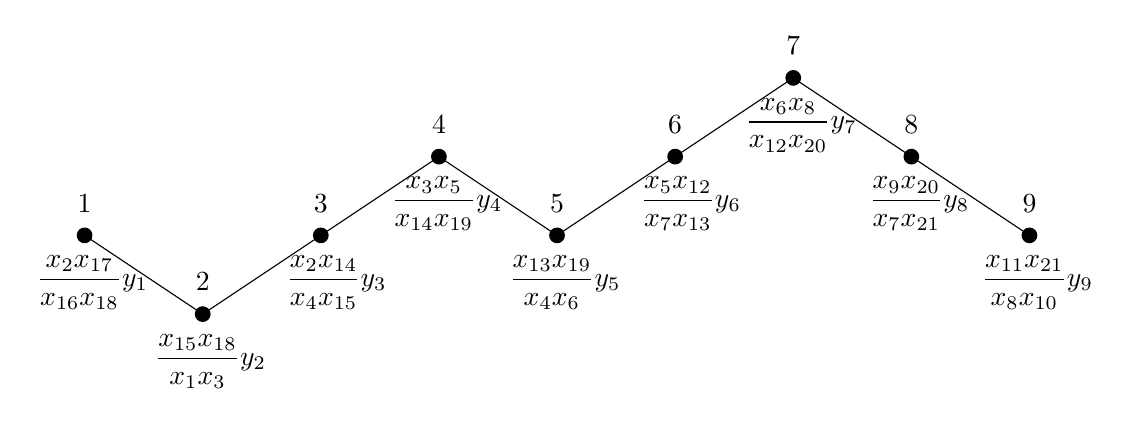
\begin{tikzpicture}
\draw (0,0)--(1.5,-1)--(4.5,1)--(6,0)--(9,2)--(12,0); %--(13.5,1)
\fill (0,0) circle(.1) node[above,yshift=.17cm] {$1$} ;
\draw (.1,-.6) node{$\displaystyle \frac{x_2 x_{17}}{x_{16}x_{18}} y_1$} ;
\fill (1.5,-1) circle(.1) node[above,yshift=.17cm] {$2$} ;
\draw (1.6,-1.6) node{$\displaystyle \frac{x_{15} x_{18}}{x_1 x_{3}}y_2$};
\fill (3,0) circle(.1) node[above,yshift=.17cm] {$3$} ;
\draw (3.2,-.6) node{$\displaystyle \frac{x_2x_{14}}{x_4x_{15}}y_3$} ;
\fill (4.5,1) circle(.1) node[above,yshift=.17cm] {$4$} ;
\draw (4.6,.4) node{$\displaystyle \frac{x_{3}x_{5}}{x_{14}x_{19}}y_4$} ;
\fill (6,0) circle(.1) node[above,yshift=.17cm] {$5$} ;
\draw (6.1,-.6) node{$\displaystyle \frac{x_{13}x_{19}}{x_{4}x_{6}}y_5$} ;
\fill (7.5,1) circle(.1) node[above,yshift=.17cm]{$6$} ;
\draw (7.7,.4) node{$\displaystyle \frac{x_{5}x_{12}}{x_7x_{13}}y_6$} ;
\fill (9,2) circle(.1) node[above,yshift=.17cm] {$7$} ;
\draw (9.1,1.4) node{$\displaystyle \frac{x_{6}x_{8}}{x_{12}x_{20}}y_7$} ;
\fill (10.5,1) circle(.1) node[above,yshift=.17cm] {$8$} ;
\draw (10.6,.4) node{$\displaystyle \frac{x_{9}x_{20}}{x_{7}x_{21}}y_8$} ;
\fill (12,0) circle(.1) node[above,yshift=.17cm] {$9$} ;
\draw (12.1,-.6) node{$\displaystyle \frac{x_{11}x_{21}}{x_{8}x_{10}}y_9$};
%\fill (13.5,1) circle(.2) node[white] {$10$} ;
%\draw (13.6,.2) node{$\displaystyle \frac{x_{9}}{x_{19}}y_{10}$} ;
\end{tikzpicture}}
	    \caption{The labeled fence poset associated to the surface from Figure~\ref{fig:sch10}.}
	    \label{fig:largefence}
	\end{figure}
  \begin{align*}
  x_{\gamma}=\displaystyle \frac{x_1x_3x_4^2x_6x_7^2x_8x_{10}x_{16}}{x_1x_2x_3x_4x_5x_6x_7x_8x_9x_{10}} \rank(P_\gamma;xy)=\displaystyle \frac{x_4x_7x_{16}}{x_2x_5x_9} \rank(P_\gamma;xy).
\end{align*}

Here, the  $\rank(P_\gamma;xy)$ consists of $64$ terms corresponding to the $64$ perfect matchings of the snake graph and a calculation by hand is impractical. There is a faster way however, which is the topic of the next section.
 \end{example}


\section{Calculating the weight polynomials via matrices}\label{sec:matrix}

\begin{table}
    \centering
    \begin{tabular}[t]{|c|c|c|}
\hline
         & Formula & Example \\
         \hline &&\\
    Addition     & &
   \\
   $\mathbf{P}\searrow\mathbf{Q}$
 &\begin{tabular}{c}
 $\rmm_w((\mathbf{P}\searrow\mathbf{Q})\!\searrow)=\rmm_w(\mathbf{P}\!\searrow) \cdot \rmm_w(\mathbf{Q}\!\searrow) $\\
 $\drm_w((\mathbf{P}\searrow\mathbf{Q})\!\nearrow)=\rmm_w(\mathbf{P}\!\searrow) \cdot \drm_w(\mathbf{Q}\!\nearrow)$
 \end{tabular}& 
 \begin{tabular}{c}
 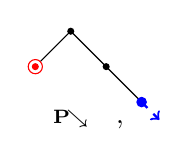
\begin{tikzpicture}[scale=.45]
\draw (0,0)--(1,1)--(3,-1);
\fill[white] (0,0) circle(.2) ;
\fill[red] (0,0) circle(.1) ;
\draw[red] (0,0) circle(.2);
\fill (1,1) circle(.1)  ;
\fill (2,0) circle(.1)  ;
\fill[blue] (3,-1) circle(.15)  ;
\draw[->, blue,dashed, thick] (3,-1)--(3.5,-1.5);
\node at (1.5,-1.5) {$\scriptstyle{\mathbf{P}\!\searrow}$\quad,};
\end{tikzpicture} \quad 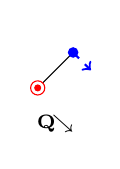
\begin{tikzpicture}[scale=.45]
\fill[white] (0,1) circle(.2) ;
\draw (0,-.5)--(1,.5);
\fill[white] (0,-.5) circle(.2) ;
\fill[red] (0,-.5) circle(.1) ;
\draw[red] (0,-.5) circle(.2);
\fill[blue] (1,.5) circle(.15)  ;
\draw[->, blue,dashed,thick] (1,.5)--(1.5,0);
\node at (.5,-1.5) {$\scriptstyle{\mathbf{Q}\!\searrow}$};
\end{tikzpicture}$\quad$ \raisebox{.2cm}{$\rightarrow$} $\quad$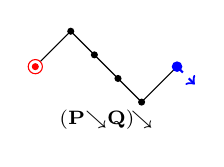
\begin{tikzpicture}[scale=.45]
\draw (0,0)--(1,1)--(3,-1)--(4,0);
\fill[white] (0,0) circle(.2) ;
\fill[red] (0,0) circle(.1) ;
\draw[red] (0,0) circle(.2);
\fill (1,1) circle(.1)  ;
\fill(1+2/3,1/3) circle(.1);
\fill (1+4/3,-1/3) circle(.1)  ;
\fill(3,-1) circle(.1);
\fill[blue] (4,0) circle(.15)  ;
\draw[->, blue,dashed, thick] (4,0)--(4.5,-.5);
\node at (2,-1.5) {$\scriptstyle{(\mathbf{P}\searrow\mathbf{Q})\!\searrow}$};
\end{tikzpicture} \end{tabular}\\ &&\\
    $\mathbf{P}\nearrow\mathbf{Q}$
        &\begin{tabular}{c}
 $\rmm_w((\mathbf{P}\nearrow\mathbf{Q})\!\searrow)=\drm_w(\mathbf{P}\!\nearrow) \cdot \rmm_w(\mathbf{Q}\!\searrow) $\\
 $\drm_w((\mathbf{P}\nearrow\mathbf{Q})\!\nearrow)=\drm_w(\mathbf{P}\!\nearrow) \cdot \drm_w(\mathbf{Q}\!\nearrow)$
 \end{tabular}&\begin{tabular}{c}
 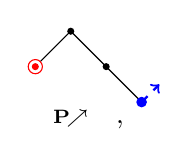
\begin{tikzpicture}[scale=.45]
\draw (0,0)--(1,1)--(3,-1);
\fill[white] (0,0) circle(.2) ;
\fill[red] (0,0) circle(.1) ;
\draw[red] (0,0) circle(.2);
\fill (1,1) circle(.1)  ;
\fill (2,0) circle(.1)  ;
\fill[blue] (3,-1) circle(.15)  ;
\draw[->, blue,dashed, thick] (3,-1)--(3.5,-.5);
\node at (1.5,-1.5) {$\scriptstyle{\mathbf{P}\!\nearrow}$\quad,};
\end{tikzpicture}\quad 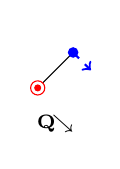
\begin{tikzpicture}[scale=.45]
\fill[white] (0,1) circle(.2) ;
\draw (0,-.5)--(1,.5);
\fill[white] (0,-.5) circle(.2) ;
\fill[red] (0,-.5) circle(.1) ;
\draw[red] (0,-.5) circle(.2);
\fill[blue] (1,.5) circle(.15)  ;
\draw[->, blue,dashed,thick] (1,.5)--(1.5,0);
\node at (.5,-1.5) {$\scriptstyle{\mathbf{Q}\!\searrow}$};
\end{tikzpicture}$\quad$ \raisebox{.2cm}{$\rightarrow$} $\quad$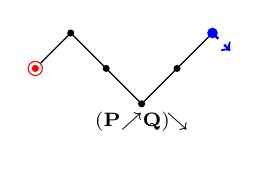
\begin{tikzpicture}[scale=.45]
\draw (0,0)--(1,1)--(3,-1)--(5,1);
\fill[white] (0,0) circle(.2) ;
\fill[red] (0,0) circle(.1) ;
\draw[red] (0,0) circle(.2);
\fill (1,1) circle(.1)  ;
\fill(2,0) circle(.1);
\fill(3,-1) circle(.1);
\fill (4,0) circle(.1) ;
\fill[blue] (5,1) circle(.15)  ;
\draw[->, blue,dashed, thick] (5,1)--(5.5,.5);
\node at (3,-1.5) {$\scriptstyle{(\mathbf{P}\nearrow\mathbf{Q})\!\searrow}$};
\end{tikzpicture} \end{tabular}\\
\hline &&\\
        Loop & &\\
        $\close(\mathbf{P}\!\searrow)$ &$\rank( \close(\mathbf{P}\!\searrow);w)=\operatorname{tr}(\rmm_w({\mathbf{P}\!\searrow}))$ &\begin{tabular}{c}
        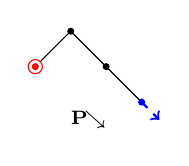
\begin{tikzpicture}[scale=.45]
\draw (0,0)--(1,1)--(3,-1);
\fill[white] (0,0) circle(.2) ;
\fill[red] (0,0) circle(.1) ;
\draw[red] (0,0) circle(.2);
\fill (1,1) circle(.1)  ;
\fill (2,0) circle(.1)  ;
\fill[blue] (3,-1) circle(.1)  ;
\draw[->, blue,dashed, thick] (3,-1)--(3.5,-1.5);
\node at (1.5,-1.5) {$\scriptstyle{\mathbf{P}\!\searrow}$};
\end{tikzpicture} $\quad$ \raisebox{.2cm}{$\rightarrow$} $\quad$   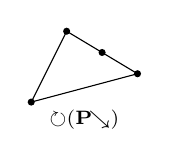
\begin{tikzpicture}[scale=.45]
\draw (0,-1)--(1,1)--(3,-.2)--(0,-1);
\fill (0,-1) circle(.1) ;
\fill (1,1) circle(.1)  ;
\fill (2,0.4) circle(.1)  ;
\fill (3,-.2) circle(.1);
\node at (1.5,-1.5) {$\scriptstyle{\close\,(\mathbf{P}\!\searrow)}$};
\end{tikzpicture}\end{tabular} \\ && \\
 $\close(\mathbf{P}\nearrow)$ &$\rank( \close(\mathbf{P}\nearrow);w)=\operatorname{tr}(\rmm_w({\mathbf{P}\!\nearrow}))$ &\begin{tabular}{c}
        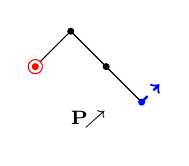
\begin{tikzpicture}[scale=.45]
\draw (0,0)--(1,1)--(3,-1);
\fill[white] (0,0) circle(.2) ;
\fill[red] (0,0) circle(.1) ;
\draw[red] (0,0) circle(.2);
\fill (1,1) circle(.1)  ;
\fill (2,0) circle(.1)  ;
\fill[blue] (3,-1) circle(.1)  ;
\draw[->, blue,dashed, thick] (3,-1)--(3.5,-.5);
\node at (1.5,-1.5) {$\scriptstyle{\mathbf{P}\!\nearrow}$};
\end{tikzpicture} $\quad$ \raisebox{.2cm}{$\rightarrow$} $\quad$   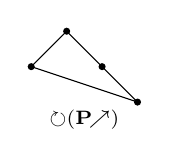
\begin{tikzpicture}[scale=.45]
\draw (0,0)--(1,1)--(3,-1)--(0,0);
\fill (0,0) circle(.1) ;
\fill (1,1) circle(.1)  ;
\fill (2,0) circle(.1)  ;
\fill (3,-1) circle(.1);
\node at (1.5,-1.5) {$\scriptstyle{\close\,(\mathbf{P}\!\nearrow)}$};
\end{tikzpicture}\end{tabular} \\
        \hline  &&\\
        Source&&\\
        Loop&&\\
             $\rhd(\mathbf{P}\!\searrow)$ &$\rmm_w( (\rhd(\mathbf{P}\!\searrow))\!\searrow) =\lloop_\searrow (\rmm_w({\mathbf{P}\!\searrow}))$ &\begin{tabular}{c}
        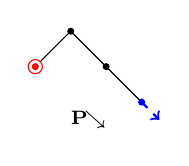
\begin{tikzpicture}[scale=.45]
\draw (0,0)--(1,1)--(3,-1);
\fill[white] (0,0) circle(.2) ;
\fill[red] (0,0) circle(.1) ;
\draw[red] (0,0) circle(.2);
\fill (1,1) circle(.1)  ;
\fill (2,0) circle(.1)  ;
\fill[blue] (3,-1) circle(.1)  ;
\draw[->, blue,dashed, thick] (3,-1)--(3.5,-1.5);
\node at (1.5,-1.5) {$\scriptstyle{\mathbf{P}\!\searrow}$};
\end{tikzpicture} $\quad$ \raisebox{.2cm}{$\rightarrow$} $\quad$   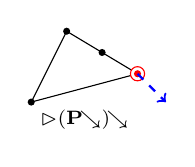
\begin{tikzpicture}[scale=.45]
\draw (0,-1)--(1,1)--(3,-.2)--(0,-1);
\fill (0,-1) circle(.1) ;
\fill (1,1) circle(.1)  ;
\fill (2,0.4) circle(.1)  ;
\fill[white] (3,-.2) circle(.2) ;
\fill[red] (3,-.2) circle(.1) ;
\draw[red] (3,-.2) circle(.2);
\draw[->, blue,dashed, thick] (3,-.2)--(3.8,-1);
\node at (1.5,-1.5) {$\scriptstyle{\rhd(\mathbf{P}\!\searrow)\!\searrow}$};
\end{tikzpicture}\end{tabular} \\ && \\
  $\rhd(\mathbf{P}\!\nearrow)$ &$\rmm_w(( \rhd(\mathbf{P}\!\nearrow))\!\searrow)=\lloop_\nearrow(
             \rmm_w({\mathbf{P}\!\nearrow}))$
  &\begin{tabular}{c}
        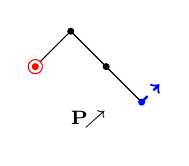
\begin{tikzpicture}[scale=.45]
\draw (0,0)--(1,1)--(3,-1);
\fill[white] (0,0) circle(.2) ;
\fill[red] (0,0) circle(.1) ;
\draw[red] (0,0) circle(.2);
\fill (1,1) circle(.1)  ;
\fill (2,0) circle(.1)  ;
\fill[blue] (3,-1) circle(.1)  ;
\draw[->, blue,dashed, thick] (3,-1)--(3.5,-.5);
\node at (1.5,-1.5) {$\scriptstyle{\mathbf{P}\!\nearrow}$};
\end{tikzpicture} $\quad$ \raisebox{.2cm}{$\rightarrow$} $\quad$   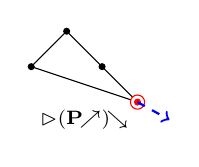
\begin{tikzpicture}[scale=.45]
\draw (0,0)--(1,1)--(3,-1)--(0,0);
\fill (0,0) circle(.1) ;
\fill (1,1) circle(.1)  ;
\fill (2,0) circle(.1)  ;
\fill[white] (3,-1) circle(.2) ;
\fill[red] (3,-1) circle(.1) ;
\draw[red] (3,-1) circle(.2);
\draw[->, blue,dashed, thick] (3,-1)--(3.9,-1.5);
\node at (1.5,-1.5) {$\scriptstyle{\rhd(\mathbf{P}\!\nearrow)\!\searrow}$};
\end{tikzpicture}\end{tabular} \\
        \hline  &&\\
        Target&&\\
        Loop&&\\
             $\lhd(\mathbf{P}\!\searrow)$ &$\rmm_w( (\lhd(\mathbf{P}\!\searrow))\!\searrow)=\rloop(\rmm_w({\mathbf{P}\!\searrow}))$ &\begin{tabular}{c}
        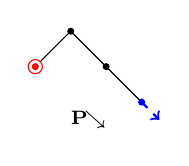
\begin{tikzpicture}[scale=.45]
\draw (0,0)--(1,1)--(3,-1);
\fill[white] (0,0) circle(.2) ;
\fill[red] (0,0) circle(.1) ;
\draw[red] (0,0) circle(.2);
\fill (1,1) circle(.1)  ;
\fill (2,0) circle(.1)  ;
\fill[blue] (3,-1) circle(.1)  ;
\draw[->, blue,dashed, thick] (3,-1)--(3.5,-1.5);
\node at (1.5,-1.5) {$\scriptstyle{\mathbf{P}\!\searrow}$};
\end{tikzpicture} $\quad$ \raisebox{.2cm}{$\rightarrow$} $\quad$   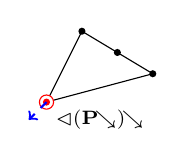
\begin{tikzpicture}[scale=.45]
\draw (0,-1)--(1,1)--(3,-.2)--(0,-1);
\fill (3,-.2) circle(.1) ;
\fill (1,1) circle(.1)  ;
\fill (2,0.4) circle(.1)  ;
\fill[white] (0,-1) circle(.2) ;
\fill[red] (0,-1) circle(.1) ;
\draw[red] (0,-1) circle(.2);
\draw[->, blue,dashed, thick] (0,-1)--(-.5,-1.5);
\node at (1.5,-1.5) {$\scriptstyle{\lhd(\mathbf{P}\!\searrow)\!\searrow}$};
\end{tikzpicture}\end{tabular} \\ && \\
  $\lhd(\mathbf{P}\!\nearrow)$ &$\rmm_w( (\lhd(\mathbf{P}\!\nearrow))\!\searrow)=\rloop (\rmm_w({\mathbf{P}\!\nearrow}))$
  &\begin{tabular}{c}
        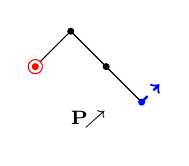
\begin{tikzpicture}[scale=.45]
\draw (0,0)--(1,1)--(3,-1);
\fill[white] (0,0) circle(.2) ;
\fill[red] (0,0) circle(.1) ;
\draw[red] (0,0) circle(.2);
\fill (1,1) circle(.1)  ;
\fill (2,0) circle(.1)  ;
\fill[blue] (3,-1) circle(.1)  ;
\draw[->, blue,dashed, thick] (3,-1)--(3.5,-.5);
\node at (1.5,-1.5) {$\scriptstyle{\mathbf{P}\!\nearrow}$};
\end{tikzpicture} $\quad$ \raisebox{.2cm}{$\rightarrow$} $\quad$   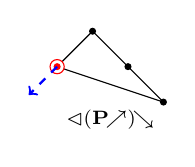
\begin{tikzpicture}[scale=.45]
\draw (0,0)--(1,1)--(3,-1)--(0,0);
\fill (0,0) circle(.1) ;
\fill (1,1) circle(.1)  ;
\fill (2,0) circle(.1)  ;
\fill (3,-1) circle(.1)  ;
\fill[white] (0,0) circle(.2) ;
\fill[red] (0,0) circle(.1) ;
\draw[red] (0,0) circle(.2);
\draw[->, blue,dashed, thick] (0,0)--(-.8,-.8);
\node at (1.5,-1.5) {$\scriptstyle{\lhd(\mathbf{P}\!\nearrow)\!\searrow}$};
\end{tikzpicture}\end{tabular} \\
\hline
    \end{tabular}
    \caption{The moves are shown through examples}
    \label{table:tableofmoves}
\end{table}

In this section, we will describe a method of calculating weight polynomials of posets with matrix multiplication.  
 An \definition{oriented poset} $\mathbf{P}=(P,x_L,x_R)$ consists of a poset $P$ with two specialized vertices $x_L$ and $x_R$ which can be thought as the left and right vertex, or alternatively the \definition{target vertex} $\target\,$  and the \definition{source vertex} $\rightarrow$. Oriented matrices actually behave like building blocks, in the sense that we connect the target of one with the arrow of another to build a larger structure. Also as building blocks, one can start with the smallest of pieces (a one element poset) to build a myriad of structures. One key difference is, there are two ways of an arrow vertex connecting with a target vertex. We can either connect via $x_R \succeq y_L$ ($x_R\nearrow y_L$) to get $\mathbf{P}\nearrow\mathbf{Q}$ or connect via $x_R \preceq y_L$ ($x_R\searrow y_L$) to get $\mathbf{P}\searrow\mathbf{Q}$.

On the weight polynomial level, we will try to streamline these operations into $2\times2$ matrices that keep track of the end points as well as the weight polynomials.  A \definition{weight matrix} of an oriented poset $\mathbf{P}$ can be thought of as an oriented matrix with an upwards or downwards pointing tail coming out of the arrow vertex. The two types of connections necessitate us to define two kinds of weight matrices.
\begin{itemize}
    \item \emph{Down pointing weight matrix of $\mathbf{P}$}: $$\displaystyle \rmm_w(\mathbf{P}\!\searrow):=\begin{bmatrix} \rank(\mathbf{P};w) & -\rank(\mathbf{P};q)|_{x_R\in I}\\ \rank(\mathbf{P};w)|_{x_L \notin I} & -\rank(\mathbf{P};w)|_{\substack{x_R\in I\\x_L \notin I}}
		\end{bmatrix}$$
    \item  \emph{Up pointing weight matrix of $\mathbf{P}$}: 
    $$	\displaystyle \drm_w(\mathbf{P}\!\nearrow):=\begin{bmatrix} \rank(\mathbf{P};w)|_{x_R\in I} & \rank(\mathbf{P};w)|_{x_R\notin I}\\ \rank(\mathbf{P};w)|_{\substack{x_R\in I\\x_L \notin I}} & \rank(\mathbf{P};w)|_{\substack{x_R\notin I\\x_L \notin I}}
			\end{bmatrix}$$
\end{itemize}
The entries are the weight polynomials of the ideals satisfying the given constraints.
We can easily go from one to the other via the \definition{tail flip} matrix $\tf=\begin{bmatrix}
				1&-1\\1&0
			\end{bmatrix}$:
		$$\drm_w(\mathbf{P}\!\nearrow)=\rmm_w(\mathbf{P}\!\searrow) \cdot \tf, \qquad \qquad \rmm_w(\mathbf{P}\!\searrow)=\drm_w(\mathbf{P}\!{\nearrow}) \cdot \tf^{-1}.$$

If we know a weight matrix of an oriented poset, we can easily read the rank polynomial off from it. For $\rmm_w(\mathbf{P}\!\searrow)$ it is given by the top left entry of the matrix and for $\drm_w(\mathbf{P}\!\nearrow)$ it is given by the sum of the entries in the top row. As we are primarily concerned with the weight polynomials for the expansion formulae calculation, it is sufficient to calculate either matrix. 
		
	\begin{figure}[ht]
	    \centering
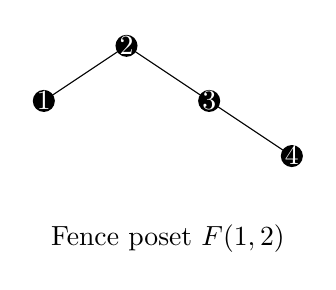
\begin{tikzpicture}[scale=.7]
\draw (0,0)--(1.5,1)--(4.5,-1);
\fill (0,0) circle(.2) node[white] {$1$} ;
\fill (1.5,1) circle(.2) node[white] {$2$} ;
\fill (3,0) circle(.2) node[white] {$3$} ;
\fill (4.5,-1) circle(.2) node[white] {$4$} ;
\node at (2.25,-2.5) {Fence poset $F(1,2)$};
\end{tikzpicture}\qquad \qquad \begin{tikzpicture}[scale=.7]
\draw (0,0)--(1.5,1)--(4.5,-1);
\fill[white] (0,0) circle(.2) ;
\fill[red] (0,0) circle(.1) ;
\draw[red] (0,0) circle(.2);
\fill (1.5,1) circle(.1)  ;
\fill (3,0) circle(.1)  ;
\fill[blue] (4.5,-1) circle(.15)  ;
\draw[->, blue,dashed] (4.5,-1)--(5.5,-5/3);
\node at (2.25,-2.5) {$\mathbf{(1,2)}\!\searrow$};
\end{tikzpicture}
\qquad  \begin{tikzpicture}[scale=.7]
\draw (0,0)--(1.5,1)--(4.5,-1);
\fill[white] (0,0) circle(.2) ;
\fill[red] (0,0) circle(.1) ;
\draw[red] (0,0) circle(.2);
\fill (1.5,1) circle(.1)  ;
\fill (3,0) circle(.1)  ;
\fill[blue] (4.5,-1) circle(.15)  ;
\draw[->, blue,dashed] (4.5,-1)--(5.5,-1/3);
\node at (2.25,-2.5) {$\mathbf{(1,2)}\!\nearrow$};
\end{tikzpicture}
\caption{One can think of the fence poset for $(1,2)$ as an oriented poset by specifying left and right end points.}\label{fig:21example}
\end{figure}

\begin{example} The fence poset of $(1,2)$ can be oriented by taking vertex $1$ as the target vertex, and vertex $4$ as the source vertex. There are two ways to add a tail to the source vertex (see Figure~\ref{fig:21example}) and the corresponding weight matrices are given below:

\begin{align*}
    \rmm_w(\mathbf{(1,2)}\!\searrow)&=\begin{bmatrix}
    \scriptstyle{1+w_1+w_4+w_1w_4+w_3w_4+w_1w_3w_4+w_1w_2w_3w_4} &  \scriptstyle{-w_4-w_1w_4-w_3w_4-w_1w_3w_4-w_1w_2w_3w_4}\\
     \scriptstyle{1+w_4+w_3w_4}&  \scriptstyle{-w_4-w_3w_4}
    \end{bmatrix},\\
        \drm_w(\mathbf{(1,2)}\!\nearrow)&=\begin{bmatrix}
    \scriptstyle{\qquad  w_4+w_1w_4+w_3w_4+w_1w_3w_4+w_1w_2w_3w_4} \qquad &  \hspace{20mm}\scriptstyle{1+w_1}\hspace{20 mm}\\
     \scriptstyle{w_4+w_3w_4}&  \scriptstyle{1}
    \end{bmatrix}.
\end{align*}

The weight polynomial of the fence poset $F(1,2)$ is equal to $1+w_1+w_4+w_1w_4+w_3w_4+w_1w_3w_4+w_1w_2w_3w_4$. It can be calculated by looking at top left entry of $\rmm_w(\mathbf{(1,2)}\!\searrow)$ or the sum of the entries in the top row of 
$\drm_w(\mathbf{(1,2)}\!\nearrow)$.
\end{example}

All fence posets can be constructed combining  a single vertex posets by up and down steps. We will use the following notation for the corresponding weight matrices:
\begin{align*}
\rmm_w(\bullet\!\searrow):=\mdo(w)=\mdom{w},\quad \qquad \drm_w(\bullet\!\nearrow):=\mup(w):=\mupm{w}.
\end{align*}
To build the posets necessary for our calculations, we will need only the two above matrices and an additional operation. Given an oriented poset, one may want to connect its source vertex to its target vertex, creating a loop. 

If the poset is completed, and no additional connections are necessary, one can simply do this by taking the trace of the corresponding matrix. We denote the poset obtained from $\mathbf{P}$ by connecting the source to the target via $x_L\preceq x_R$ (respectively $x_L\succeq x_R$) by $\close(\mathbf{P}\!\searrow)$ (respectively $\close(\mathbf{P}\!\nearrow)$.

This is a poset that is not oriented. If no more connections are necessary, as in the case of circular fence posets corresponding to the band graphs, it is enough to use the trace operation to calculate the corresponding weight polynomial:

\begin{align*}
    \rank( \close(\mathbf{P}\!\searrow);w)&=\operatorname{tr}(\rmm_w({\mathbf{P}\!\searrow})),\\
    \rank( \close(\mathbf{P}\!\nearrow);w)&=\operatorname{tr}(\rmm_w({\mathbf{P}\!\nearrow})).
\end{align*}

The proofs of the above identities are given in \cite{O22} where oriented posets are originally defined. Although that work is concerned with rank polynomials and not weight polynomials, the same ideas apply. We will only include proofs for the new constructions given below.

When we want to continue making connections to a loop  from the source vertex, we use the source loop operation. The \definition{source loop} of $\mathbf{P}\!\searrow$ is the oriented poset $(\close(\mathbf{P}\!\searrow),x_R,x_R)$. We denote it by $\rhd(\mathbf{P}\!\searrow)$. We can similarly define $\rhd(\mathbf{P}\!\nearrow)$. 

Calculating the weight matrix of a source loop requires a separate function as we are altering our source and target matrices.

\begin{align*}
    \lloop_\searrow\left( \begin{bmatrix}
    a&b\\c&d
    \end{bmatrix}\right):&=& \begin{bmatrix}
    a+d& b-d\\a+b&0
    \end{bmatrix} \qquad \qquad     \lloop_\nearrow\left( \begin{bmatrix}
    a&b\\c&d
    \end{bmatrix}\right):&=&  \begin{bmatrix}
    a+d& -a\\d&0
    \end{bmatrix}
\end{align*}

\begin{thm}~\label{theorem1} The weight matrices correponding to $\rhd(\mathbf{P}\!\searrow)$ and $\rhd(\mathbf{P}\!\nearrow)$ can be calculated via the $\lloop$ functions as follows: 
\begin{align*}
    \lloop_\searrow(\rmm_w(\mathbf{P}\!\searrow))&= \rmm_w( (\rhd(\mathbf{P}\!\searrow))\!\searrow), \qquad 
    \lloop_\nearrow(\drm_w(\mathbf{P}\!\nearrow))= \rmm_w( (\rhd(\mathbf{P}\!\nearrow))\!\nearrow).
\end{align*}
\end{thm}
\begin{proof} Consider the entries of the matrix $\rmm_w( (\rhd(\mathbf{P}\!\searrow))\!\searrow)$. As the poset has an added connection $x_R\succeq x_L$, the top left corner is given by the trace of $\rmm_w(\mathbf{P}\!\searrow)$, which matches the top left entry of $\lloop_\searrow$. The top right corner is generated by all the ideals of this poset that contain the source vertex $x_R$, times $(-1)$. As the ideals that contain $x_R$ also contain $x_L$ by the relation $x_R\succeq x_L$, we have all the ideals of our original poset that contain $x_L$ minus the ideals that contain $x_L$ but not $x_R$, multiplied by $(-1)$. That is the top right entry minus the bottom right entry of $\rmm_w(\mathbf{P}\!\searrow)$. For the bottom left entry of $\rmm_w( (\rhd(\mathbf{P}\!\searrow))\!\searrow)$, we need the weight polynomial generated by the ideals containing the target vertex, which is also $x_R$. These remain unaffected by $x_R\succeq x_L$, so we can just read them of from the top right entry of $\rmm_w(\mathbf{P}\!\searrow)$, multiplied by $(-1)$. Finally, as the source and target vertices are the same, the bottom right entry must be $0$. The entries of $\rmm_w( (\rhd(\mathbf{P}\!\searrow))\!\searrow)$ can be similarly computed.
\end{proof}

We can also define the target loop operation, where any further connections are made using the target (left) vertex. The \definition{target loop} of $\mathbf{P}\!\searrow$ is the oriented poset $(\close(\mathbf{P}\!\searrow),x_L,x_L)$, denoted by $\lhd(\mathbf{P}\!\searrow)$. The target loop  $\lhd(\mathbf{P}\!\nearrow)$ is similarly defined. 

For the target loop, the direction of the loop does not change the function, so one function is sufficent.

\begin{align*}
    \rloop\left( \begin{bmatrix}
    a&b\\c&d
    \end{bmatrix}\right): =& \begin{bmatrix}
    a+d& c-a\\c+d&0
    \end{bmatrix}
\end{align*}

\begin{thm}~\label{theorem2} The weight matrices correponding to $\rhd(\mathbf{P}\!\searrow)$ and $\rhd(\mathbf{P}\!\nearrow)$ can be calculated via the $\lloop$ functions as follows: 
\begin{align*}
    \rloop(\rmm_w(\mathbf{P}\!\searrow))&= \rmm_w( (\lhd(\mathbf{P}\!\searrow))\!\searrow), \qquad 
    \rloop-(\drm_w(\mathbf{P}\!\nearrow))= \rmm_w( (\lhd(\mathbf{P}\!\nearrow))\!\nearrow).
\end{align*}
\end{thm}
\begin{proof}One can calculate coordinate by coordinate as in the source loop case. 
\end{proof}



Combining Theorem~\ref{theorem1} and Theorem~\ref{theorem2} with Proposition~\ref{proposition}, we can compute the cluster expansion formulae for arcs by matrix multiplications.

See Table~\ref{table:tableofmoves} for a list of all the operations listed above, their formulas and examples. 






\section{Example Calculations}

In this section, we will illustrate the techniques described above through different kinds of examples that come up in the setting of cluster algebras. We will show how posets corresponding to arcs can be built step by step via matrices, and how the corresponding expansion formula can be calculated in each case. Note that though we keep our attention to posets corresponding to snake, band and loop graphs, the methods are actually adaptable to a variety of settings.

\subsection{Fence posets with no loops}

If the fence poset corresponding to our arc has no loops, we can build it using rank up and down steps only, where the direction of the matrix for vertex $i$ is determined by the direction of the connection between $i$ and $i+1$. We will always use the down pointing matrix for the final vertex as a convention.

Consider the arc from Example~\ref{ex:noloop2}, accompanied by Figures~\ref{fig:sch10} and \ref{fig:largefence}. 
The underlying fence can be built by combining up and down steps as follows:
\begin{center} \scalebox{.8}{
\begin{tikzpicture}
\draw[->, blue, dashed, thick] (0,0)--(1,-2/3);
\draw[->, blue, dashed, thick] (1.5,-1)--(2.5,-1/3);
\draw[->, blue, dashed, thick] (3,0)--(4,2/3);
\draw[->, blue, dashed, thick] (4.5,1)--(5.5,1/3);
\draw[->, blue, dashed, thick] (6,0)--(7,2/3);
\draw[->, blue, dashed, thick] (7.5,1)--(8.5,5/3);
\draw[->, blue, dashed, thick] (9,2)--(10,4/3);
\draw[->, blue, dashed, thick] (10.5,1)--(11.5,1/3);
\draw[->, blue, dashed, thick] (12,0)--(13,-2/3);
\fill (0,0) circle(.2) node[white] {$1$} ;
\draw (.1,-.5) node{$\displaystyle w_1$} ;%
\fill (1.5,-1) circle(.2) node[white] {$2$} ;
\draw (1.6,-1.5) node{$\displaystyle w_2$} ;
\fill (3,0) circle(.2) node[white] {$3$} ;
\draw (3.1,-.5) node{$\displaystyle w_3$} ;
\fill (4.5,1) circle(.2) node[white] {$4$} ;
\draw (4.6,.5) node{$\displaystyle w_4$} ;
\fill (6,0) circle(.2) node[white] {$5$} ;
\draw (6.1,-.5) node{$\displaystyle w_5$} ;
\fill (7.5,1) circle(.2) node[white] {$6$} ;
\draw (7.6,.5) node{$\displaystyle w_6$} ;
\fill (9,2) circle(.2) node[white] {$7$} ;
\draw (9.1,1.5) node{$\displaystyle w_7$} ;
\fill (10.5,1) circle(.2) node[white] {$8$} ;
\draw (10.6,.5) node{$\displaystyle w_8$} ;
\fill (12,0) circle(.2) node[white] {$9$} ;
\draw (12.1,-.5) node{$\displaystyle w_9$} ;
\fill[white] (0,0) circle(.2) ;
\fill[red] (0,0) circle(.1) ;
\draw[red] (0,0) circle(.2);
\fill[white] (1.5,-1) circle(.2) ;
\fill[red] (1.5,-1) circle(.1) ;
\draw[red] (1.5,-1) circle(.2);
\fill[white] (3,0) circle(.2) ;
\fill[red] (3,0) circle(.1) ;
\draw[red] (3,0) circle(.2);
\fill[white] (4.5,1) circle(.2) ;
\fill[red] (4.5,1) circle(.1) ;
\draw[red] (4.5,1) circle(.2);
\fill[white] (6,0) circle(.2) ;
\fill[red] (6,0) circle(.1) ;
\draw[red] (6,0) circle(.2);
\fill[white] (7.5,1) circle(.2) ;
\fill[red] (7.5,1) circle(.1) ;
\draw[red] (7.5,1) circle(.2);
\fill[white] (9,2) circle(.2) ;
\fill[red] (9,2) circle(.1) ;
\draw[red] (9,2) circle(.2);
\fill[white] (10.5,1) circle(.2) ;
\fill[red] (10.5,1) circle(.1) ;
\draw[red] (10.5,1) circle(.2);
\fill[white] (12,0) circle(.2) ;
\fill[red] (12,0) circle(.1) ;
\draw[red] (12,0) circle(.2);
\end{tikzpicture}}
\end{center}
\begin{comment} The underlying fence is depicted below.\begin{center}
    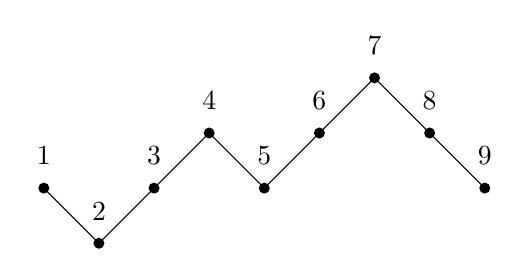
\begin{tikzpicture}[scale=.7]
\draw (0,0)--(1,-1)--(3,1)--(4,0)--(6,2)--(8,0); %--(13.5,1)
\fill (0,0) circle(.1) node[above,yshift=.17cm] {$1$} ;
\fill (1,-1) circle(.1) node[above,yshift=.17cm] {$2$} ;
\fill (2,0) circle(.1) node[above,yshift=.17cm] {$3$} ;
\fill (3,1) circle(.1) node[above,yshift=.17cm] {$4$} ;
\fill (4,0) circle(.1) node[above,yshift=.17cm] {$5$} ;
\fill (5,1) circle(.1) node[above,yshift=.17cm]{$6$} ;
\fill (6,2) circle(.1) node[above,yshift=.17cm] {$7$} ;
\fill (7,1) circle(.1) node[above,yshift=.17cm] {$8$} ;
\fill (8,0) circle(.1) node[above,yshift=.17cm] {$9$} ;
\end{tikzpicture}
\end{center}\end{comment}

The corresponding matrix is given by: $\mdo(w_1)\mup(w_2)\mup(w_3)\mdo(w_4)\mup(w_5)\mup(w_6)\mdo(w_7)\mdo(w_8)\mdo(w_9)$.

This can be expressed as a matrix product as follows:

\vspace{2mm}

\scalebox{.85}{$\mdom{w_1}\mupm{w_2}\mupm{w_3}\mdom{w_4}\mupm{w_5}\mupm{w_6}\mdom{w_7}\mdom{w_8}\mdom{w_9}$.}

\vspace{2mm}

The upper left entry gives us the weight polynomial $\rank(P_\gamma;w)$.

\begin{dmath*}
\rank(P_\gamma;w)=
1+ w_2 + w_5 + w_9 + w_1w_2 + w_2w_3 + w_2w_5 + w_5w_6 + w_2w_9 + w_5w_9 + w_8w_9 + w_1w_2w_3 + w_1w_2w_5 + w_2w_3w_5 + w_2w_5w_6 + w_1w_2w_9 + w_2w_3w_9 + w_2w_5w_9 + w_5w_6w_9 + w_2w_8w_9 + w_5w_8w_9  + w_1w_2w_3w_5 + w_2w_3w_4w_5 + w_1w_2w_5w_6 + w_2w_3w_5w_6 + w_1w_2w_3w_9 + w_1w_2w_5w_9 + w_2w_3w_5w_9 + w_2w_5w_6w_9 + w_1w_2w_8w_9 + w_2w_3w_8w_9 + w_2w_5w_8w_9 + w_5w_6w_8w_9 + w_1w_2w_3w_4w_5 + w_1w_2w_3w_5w_6 + w_2w_3w_4w_5w_6 + w_1w_2w_3w_5w_9 + w_2w_3w_4w_5w_9 + w_1w_2w_5w_6w_9 + w_2w_3w_5w_6w_9 + w_1w_2w_3w_8w_9 + w_1w_2w_5w_8w_9 + w_2w_3w_5w_8w_9 + w_2w_5w_6w_8w_9 + w_5w_6w_7w_8w_9 + w_1w_2w_3w_4w_5w_6 + w_1w_2w_3w_4w_5w_9 + w_1w_2w_3w_5w_6w_9 + w_2w_3w_4w_5w_6w_9 + w_1w_2w_3w_5w_8w_9 + w_2w_3w_4w_5w_8w_9 + w_1w_2w_5w_6w_8w_9 + w_2w_3w_5w_6w_8w_9 + w_2w_5w_6w_7w_8w_9  + w_1w_2w_3w_4w_5w_6w_9 + w_1w_2w_3w_4w_5w_8w_9 + w_1w_2w_3w_5w_6w_8w_9 + w_2w_3w_4w_5w_6w_8w_9 + w_1w_2w_5w_6w_7w_8w_9 + w_2w_3w_5w_6w_7w_8w_9+ w_1w_2w_3w_4w_5w_6w_8w_9 + w_1w_2w_3w_5w_6w_7w_8w_9 + w_2w_3w_4w_5w_6w_7w_8w_9
+w_1w_2w_3w_4w_5w_6w_7w_8w_9 
\end{dmath*}

We can plug in the labels from Figure~\ref{fig:largefence} in the formula below to get $64$ term expansion formula. 

 \begin{align*}
  x_{\gamma}=\displaystyle \frac{x_1x_3x_4^2x_6x_7^2x_8x_{10}}{x_1x_2x_3x_4x_5x_6x_7x_8x_9x_{10}} \rank(P_\gamma;xy)=\displaystyle \frac{x_4x_7}{x_2x_5x_9} \rank(P_\gamma;xy).
\end{align*}

Note that while looking at larger triangulations increases the number of matchings exponentially, in the matrix expansion it just corresponds to adding one more matrix per triangle. 

\subsection{Band graph} Band graphs are obtained by considering the closed curves on the surfaces. We can create their associated snake graphs by identifying a boundary edge of the first tile with a boundary edge of the last tile, where both edges have the same sign. 

Consider the following is an example of a closed arc on a surface of an annulus with initial triangulation with five arcs, depicted in Figure~\ref{fig:band}. It shows the corresponding band graph with the fence poset drawn.  

\begin{figure}[H]
\includegraphics[width=13cm]{images/glued_band.png}
\caption{A closed arc with the corresponding band graph, poset and labeled poset. The marked edges in the band graph are glued.} \label{fig:band}
\end{figure}



One can build the corresponding oriented poset by combining up and down steps, and than taking the trace to connect the two ends.

\begin{center} \scalebox{.8}{
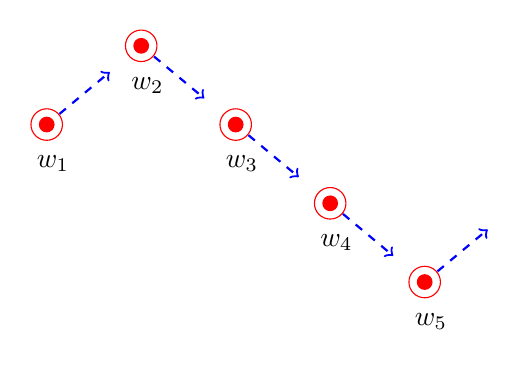
\begin{tikzpicture}
\draw[->, blue, dashed, thick] (7.5*.8,1)--(8.5*.8,5/3);
\draw[->, blue, dashed, thick] (9*.8,2)--(10*.8,4/3);
\draw[->, blue, dashed, thick] (10.5*.8,1)--(11.5*.8,1/3);
\draw[->, blue, dashed, thick] (12*.8,0)--(13*.8,-2/3);
\draw[->, blue, dashed, thick] (13.5*.8,-1)--(14.5*.8,-1/3);
\fill (7.5*.8,1) circle(.2) node[white] {$6$} ;
\draw (7.6*.8,.5) node{$\displaystyle w_1$} ;
\fill (9*.8,2) circle(.2) node[white] {$7$} ;
\draw (9.1*.8,1.5) node{$\displaystyle w_2$} ;
\fill (10.5*.8,1) circle(.2) node[white] {$8$} ;
\draw (10.6*.8,.5) node{$\displaystyle w_3$} ;
\fill (12*.8,0) circle(.2) node[white] {$9$} ;
\draw (12.1*.8,-.5) node{$\displaystyle w_4$} ;
\fill (12*.8,0) circle(.2) node[white] {$9$} ;
\draw (13.6*.8,-1.5) node{$\displaystyle w_5$} ;
\fill[white] (7.5*.8,1) circle(.2) ;
\fill[red] (7.5*.8,1) circle(.1) ;
\draw[red] (7.5*.8,1) circle(.2);
\fill[white] (9*.8,2) circle(.2) ;
\fill[red] (9*.8,2) circle(.1) ;
\draw[red] (9*.8,2) circle(.2);
\fill[white] (10.5*.8,1) circle(.2) ;
\fill[red] (10.5*.8,1) circle(.1) ;
\draw[red] (10.5*.8,1) circle(.2);
\fill[white] (12*.8,0) circle(.2) ;
\fill[red] (12*.8,0) circle(.1) ;
\draw[red] (12*.8,0) circle(.2);
\fill[white] (13.5*.8,-1) circle(.2) ;
\fill[red] (13.5*.8,-1) circle(.1) ;
\draw[red] (13.5*.8,-1) circle(.2);
\end{tikzpicture}
 \raisebox{15mm}{ \raisebox{.4cm}{\scalebox{2}{$\Rightarrow$}}}
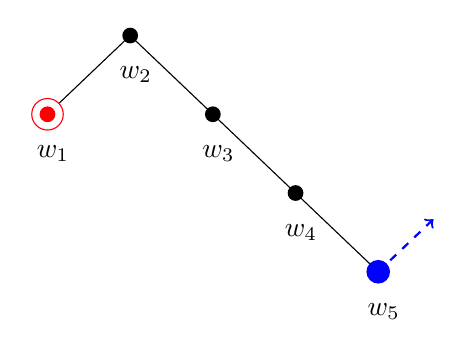
\begin{tikzpicture}
\draw (7.5*.7,1)--(9*.7,2)--(13.5*.7,-1);
\draw[->, blue, dashed, thick] (13.5*.7,-1)--(14.5*.7,-1/3);
\fill (7.5*.7,1) circle(.1) ;
\draw (7.6*.7,.5) node{$\displaystyle w_1$} ;
\fill (9*.7,2) circle(.1) ;
\draw (9.1*.7,1.5) node{$\displaystyle w_2$} ;
\fill (10.5*.7,1) circle(.1) ;
\draw (10.6*.7,.5) node{$\displaystyle w_3$} ;
\fill (12*.7,0) circle(.1) ;
\draw (12.1*.7,-.5) node{$\displaystyle w_4$} ;
\fill[blue] (13.5*.7,-1) circle(.15);
\draw (13.6*.7,-1.5) node{$\displaystyle w_5$} ;
\fill[white] (7.5*.7,1) circle(.2) ;
\fill[red] (7.5*.7,1) circle(.1) ;
\draw[red] (7.5*.7,1) circle(.2);
\end{tikzpicture}
 \raisebox{15mm}{\raisebox{.4cm}{\scalebox{2}{$\Rightarrow$}} }
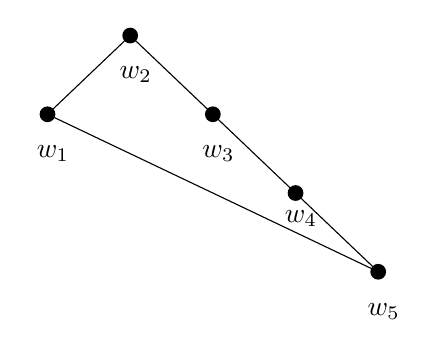
\begin{tikzpicture}
\draw (7.5*.7,1)--(9*.7,2)--(13.5*.7,-1)--(7.5*.7,1);
\fill (7.5*.7,1) circle(.1);
\draw (7.6*.7,.5) node{$\displaystyle w_1$};
\fill (9*.7,2) circle(.1);
\draw (9.1*.7,1.5) node{$\displaystyle w_2$};
\fill (10.5*.7,1) circle(.1);
\draw (10.6*.7,.5) node{$\displaystyle w_3$};
\fill (12*.7,0) circle(.1);
\draw (12.1*.7,-.5) node[below,yshift=.4cm]{$\displaystyle w_4$};
\fill (13.5*.7,-1) circle(.1);
\draw (13.6*.7,-1.5) node{$\displaystyle w_5$};
\end{tikzpicture}}
\end{center}

We get the following formula for the rank polynomial:
\begin{align*}
 \rank(P_\gamma;xy)&=   \operatorname{tr}(\mup(w_1)\mdo(w_2)\mdo(w_3)\mdo(w_4)\mup(w_5))\\
    &=\operatorname{tr}\left(\mupm{w_1}\mdom{w_2}\mdom{w_3}\mdom{w_4}\mupm{w_5}\right)\\
    &=1+w_5+w_1w_5+w_4w_5+w_1w_4w_5+w_3w_4w_5+w_1w_3w_4w_5+w_1w_2w_3w_4w_5.
\end{align*}

As the minimal matching has the $x$ value $x_1x_2^2x_3x_4$, the expansion formula is as follows:
\begin{dmath*}x_{\gamma}=\displaystyle {\frac{x_1x_2^2x_3x_4}{x_1x_2x_3x_4x_5}} \rank(P_\gamma;xy)=\frac{x_2}{x_5}+\frac{x_2x_6x_8}{x_1x_4x_5}y_5+\frac{x_7x_8}{x_1x_4}y_1y_5+\frac{x_2x_5x_6x_{10}}{x_1x_3x_4}y_4y_5+\frac{x_5^2x_7x_{10}}{x_1x_3x_4}y_1y_4y_5+\frac{x_4x_5x_6x_{9}}{x_1x_3x_4}y_3y_4y_5+\frac{x_5^2x_7x_{9}}{x_1x_2x_3}y_1y_3y_4y_5+\frac{x_5^2}{x_2}y_1y_2y_3y_4y_5.
\end{dmath*}
\subsection{Loop graph}

To build the fence poset corresponding to a loop graph, we will need the above operations as well as the source and target loop operations whenever they are necessary. We will do step by step calculations for three examples: one with a single notched arch, and two with double notched arches.

\begin{example}\label{ex:single} Consider the arc given in Figure~\ref{singlenotched}, also considered in \cite{wilson}.

\begin{figure}[H]
\includegraphics[width=13cm]{images/single_glued.png}
\caption{An example with a single notched arc, from \cite{wilson}, with corresponding loop graph, poset and labeled poset.} \label{singlenotched}
\end{figure}


  
Let us build the underlying poset step by step to get the weight polynomial.


\vspace{5 mm}

\noindent{\textbf{Step $1$: }} We connect the first four vertices with appropriate arrows. We use the upwards arrow for vertex $4$ because we will connect it to node $1$ by adding the relation $1\succeq 4$ in step 2.

\begin{figure}[H]
    \centering
    \scalebox{.8}{
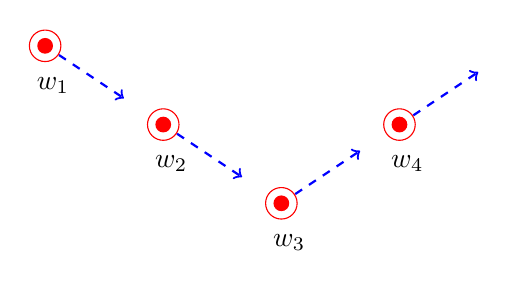
\begin{tikzpicture}
\draw[->, blue, dashed, thick] (0,0)--(1,-2/3);
\draw[->, blue, dashed, thick] (1.5,-1)--(2.5,-5/3);
\draw[->, blue, dashed, thick] (3,-2)--(4,-4/3);
\draw[->, blue, dashed, thick] (4.5,-1)--(5.5,-1/3);
\fill (0,0) circle(.2) node[white] {$1$} ;
\draw (.1,-.5) node{$\displaystyle w_1$} ;%
\fill (1.5,-1) circle(.2) node[white] {$2$} ;
\draw (1.6,-1.5) node{$\displaystyle w_2$} ;
\fill (3,-2) circle(.2) node[white] {$3$} ;
\draw (3.1,-2.5) node{$\displaystyle w_3$} ;
\fill (4.5,-1) circle(.2) node[white] {$4$} ;
\draw (4.6,-1.5) node{$\displaystyle w_4$} ;
\fill[white] (0,0) circle(.2) ;
\fill[red] (0,0) circle(.1) ;
\draw[red] (0,0) circle(.2);
\fill[white] (1.5,-1) circle(.2) ;
\fill[red] (1.5,-1) circle(.1) ;
\draw[red] (1.5,-1) circle(.2);
\fill[white] (3,-2) circle(.2) ;
\fill[red] (3,-2) circle(.1) ;
\draw[red] (3,-2) circle(.2);
\fill[white] (4.5,-1) circle(.2) ;
\fill[red] (4.5,-1) circle(.1) ;
\draw[red] (4.5,-1) circle(.2);
\end{tikzpicture} \raisebox{15mm}{$\qquad$ \scalebox{2}{$\Rightarrow$} $\qquad$}
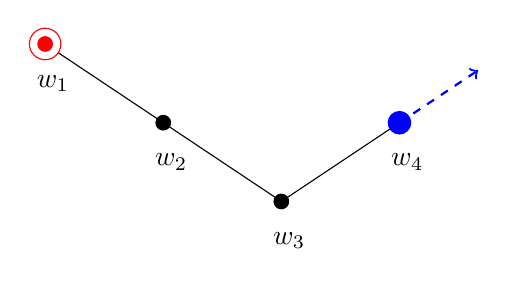
\begin{tikzpicture}
\draw (0,0)-- (3,-2)--(4.5,-1);
\draw[->, blue, dashed,thick] (4.5,-1)--(5.5,-1/3);
\fill (0,0) circle(.1) ;
\draw (.1,-.5) node{$\displaystyle w_1$} ;%
\fill (1.5,-1) circle(.1) ;
\draw (1.6,-1.5) node{$\displaystyle w_2$} ;
\fill (3,-2) circle(.1) ;
\draw (3.1,-2.5) node{$\displaystyle w_3$} ;
\fill[blue] (4.5,-1) circle(.15);
\draw (4.6,-1.5) node{$\displaystyle w_4$} ;
\fill[white] (0,0) circle(.2) ;
\fill[red] (0,0) circle(.1) ;
\draw[red] (0,0) circle(.2);
\end{tikzpicture}}
\end{figure}

%\vspace{-3mm}

The corresponding matrix is given by $\mdo(w_1)\mdo(w_2)\mup(w_3)\mup(w_4)$.
 \begin{align*}
S_{1} :=  \mdo(w_1)\mdo(w_2)\mup(w_3)\mup(w_4)= \mdom{w_1}\mdom{w_2}\mupm{w_3}\mupm{w_4}.
\end{align*}

\vspace{9 mm}

\noindent{\textbf{Step $2$: }} Now we need to connect the upwards pointing arrow from node $4$ with node $1$ to form a loop. We will use the source loop operation as we want to keep making connections using  node $4$.
\begin{figure}[H]
    \centering \scalebox{.8}{
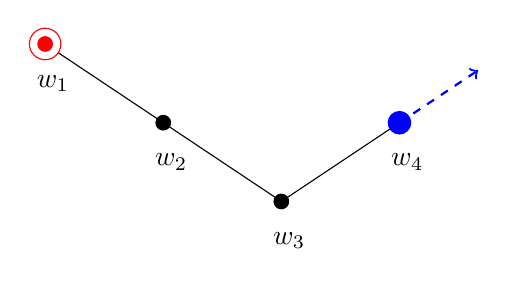
\begin{tikzpicture}
\draw (0,0)-- (3,-2)--(4.5,-1);
\draw[->, blue, dashed, thick] (4.5,-1)--(5.5,-1/3);
\fill (0,0) circle(.1) ;
\draw (.1,-.5) node{$\displaystyle w_1$} ;%
\fill (1.5,-1) circle(.1) ;
\draw (1.6,-1.5) node{$\displaystyle w_2$} ;
\fill (3,-2) circle(.1) ;
\draw (3.1,-2.5) node{$\displaystyle w_3$} ;
\fill[blue] (4.5,-1) circle(.15);
\draw (4.6,-1.5) node{$\displaystyle w_4$} ;
\fill[white] (0,0) circle(.2) ;
\fill[red] (0,0) circle(.1) ;
\draw[red] (0,0) circle(.2);
\end{tikzpicture} \raisebox{15mm}{$\qquad$ \scalebox{2}{$\Rightarrow$} $\qquad$}
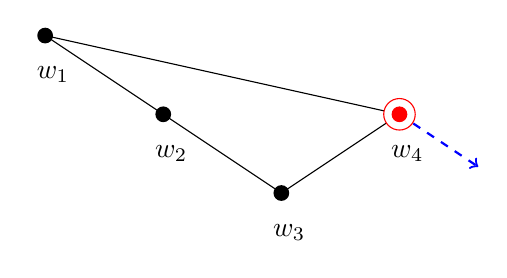
\begin{tikzpicture}
\draw (0,0)-- (3,-2)--(4.5,-1)--(0,0);
\draw[->, blue, dashed, thick] (4.5,-1)--(5.5,-5/3);
\fill (0,0) circle(.1) ;
\draw (.1,-.5) node{$\displaystyle w_1$} ;%
\fill (1.5,-1) circle(.1) ;
\draw (1.6,-1.5) node{$\displaystyle w_2$} ;
\fill (3,-2) circle(.1) ;
\draw (3.1,-2.5) node{$\displaystyle w_3$} ;
\fill[blue] (4.5,-1) circle(.15);
\draw (4.6,-1.5) node{$\displaystyle w_4$} ;
\fill[white] (4.5,-1) circle(.2) ;
\fill[red] (4.5,-1) circle(.1) ;
\draw[red] (4.5,-1) circle(.2);
\end{tikzpicture}}
\end{figure}

We get the matrix: $S_2=\lloop_\nearrow(S_1)$. The formula for $S_2$ is:
$$  \lloop_\nearrow \left( \mdo(w_1)\mdo(w_2)\mup(w_3)\mup(w_4) \right).$$

\vspace{9 mm}

\noindent{\textbf{Step $3$: }} We connect an up step for $5$ and a down step for $6$ (an up step for $6$ would also work as we are making no more connections).

\begin{figure}[H]
    \centering \scalebox{.8}{
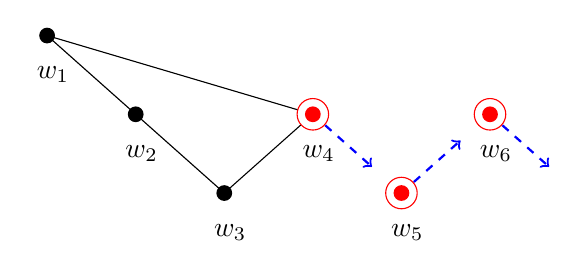
\begin{tikzpicture}
\draw (0*.75,0)-- (3*.75,-2)--(4.5*.75,-1)--(0*.75,0);
%\draw[->, blue, dotted] (4.5*.75,-1)--(5.5*.75,-1/3);
\draw[->, blue, dashed, thick] (4.5*.75,-1)--(5.5*.75,-5/3);
%\draw[black,->,thick] (5.2*.75,-3/4)--(5.2*.75,-5/4);
\fill (0*.75,0) circle(.1) ;
\draw (.1*.75,-.5) node{$\displaystyle w_1$} ;%
\fill (1.5*.75,-1) circle(.1) ;
\draw (1.6*.75,-1.5) node{$\displaystyle w_2$} ;
\fill (3*.75,-2) circle(.1) ;
\draw (3.1*.75,-2.5) node{$\displaystyle w_3$} ;
\draw (4.6*.75,-1.5) node{$\displaystyle w_4$} ;
\fill[white] (4.5*.75,-1) circle(.2) ;
\fill[red] (4.5*.75,-1) circle(.1) ;
\draw[red] (4.5*.75,-1) circle(.2);
\draw (6.1*.75,-2.5) node{$\displaystyle w_5$} ;
\draw (7.6*.75,-1.5) node{$\displaystyle w_6$} ;
\draw[->, blue, dashed, thick] (6*.75,-2)--(7*.75,-4/3);
\draw[->, blue, dashed, thick] (7.5*.75,-1)--(8.5*.75,-5/3);
\fill[white] (6*.75,-2) circle(.2) ;
\fill[red] (6*.75,-2) circle(.1) ;
\draw[red] (6*.75,-2) circle(.2);
\fill[white] (7.5*.75,-1) circle(.2) ;
\fill[red] (7.5*.75,-1) circle(.1) ;
\draw[red] (7.5*.75,-1) circle(.2);
\end{tikzpicture}
 \raisebox{15mm}{$\qquad$ \scalebox{2}{$\Rightarrow$} $\qquad$}
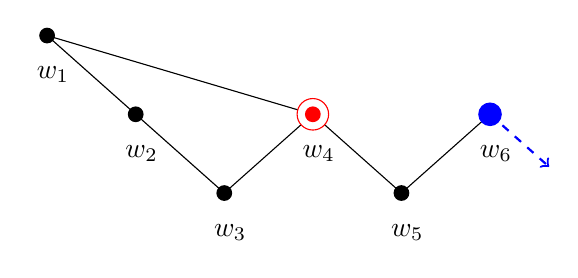
\begin{tikzpicture}
\draw (0*.75,0)-- (3*.75,-2)--(4.5*.75,-1)--(0*.75,0);
\draw(4.5*.75,-1)--(6*.75,-2)--(7.5*.75,-1);
\fill (0*.75,0) circle(.1) ;
\draw (.1*.75,-.5) node{$\displaystyle w_1$} ;%
\fill (1.5*.75,-1) circle(.1) ;
\draw (1.6*.75,-1.5) node{$\displaystyle w_2$} ;
\fill (3*.75,-2) circle(.1) ;
\draw (3.1*.75,-2.5) node{$\displaystyle w_3$} ;
\draw (4.6*.75,-1.5) node{$\displaystyle w_4$} ;
\fill[blue] (7.5*.75,-1) circle(.15) ;
\draw (6.1*.75,-2.5) node{$\displaystyle w_5$} ;
\draw (7.6*.75,-1.5) node{$\displaystyle w_6$} ;
\draw[->, blue, dashed, thick] (7.5*.75,-1)--(8.5*.75,-5/3);
\fill(6*.75,-2) circle(.1) ;
\fill[white] (4.5*.75,-1) circle(.2) ;
\fill[red] (4.5*.75,-1) circle(.1) ;
\draw[red] (4.5*.75,-1) circle(.2);
\end{tikzpicture}}
\end{figure}

We have $S_3=S_2 \cdot \tf \cdot \mup(w_5) \cdot \mdo(w_6)$. We get the following matrix expansion: \begin{align*}
&\lloop_\nearrow \left( \mdom{w_1}\mdom{w_2}\mupm{w_3}\mupm{w_4} \right) \mupm{w_5}\mdom{w_6}.
\end{align*}

The weight polynomial is given by the top left entry of the resulting matrix:
\begin{dmath*}
1+w_3+w_5+w_2w_3+w_3w_5+w_5w_6+w_2w_3w_5+w_3w_4w_5+w_3w_5w_6+w_2w_3w_4w_5+w_2w_3w_5w_6+w_3w_4w_5w_6+w_1w_2w_3w_4w_5+w_2w_3w_4w_5w_6+w_1w_2w_3w_4w_5w_6.
\end{dmath*}
 
 Now we can plug in the weights and obtain the expansion formula:
 \begin{dmath*}
 x_{\gamma}=\displaystyle {\frac{x(M_-)}{\operatorname{cross}(\gamma,T)}} \rank(P_\gamma;xy)=\frac{x_1x_2x_4^2x_6x_9}{x_1x_2x_3x_4x_5x_6}\rank(P_\gamma;xy)=\frac{x_4x_9}{x_3x_5}+\frac{x_1x_9x_{15}}{x_2x_3x_5}y_3+\frac{x_9x_{11}x_{14}}{x_3x_5x_6}y_5+\frac{x_9x_{10}}{x_2x_5}y_2y_3+\frac{x_1x_9x_{11}x_{14}x_{15}}{x_2x_3x_4x_5x_6}y_3y_5+\frac{x_{7}x_{14}}{x_3x_6}y_5y_6+\frac{x_9x_{10}x_{11}x_{14}}{x_2x_4x_5x_6}y_2y_3y_5+\frac{x_9x_{11}x_{15}}{x_2x_4x_6}y_3y_4y_5+\frac{x_1x_{7}x_{14}x_{15}}{x_2x_3x_4x_6}y_3y_5y_6+\frac{x_3x_9x_{10}x_{11}}{x_1x_2x_4x_6}y_2y_3y_4y_5+\frac{x_7x_{10}x_{14}}{x_2x_4x_6}y_2y_3y_5y_6+\frac{x_5x_{7}x_{15}}{x_2x_4x_6}y_3y_4y_5y_6+\frac{x_9x_{11}}{x_1x_6}y_1y_2y_3y_4y_5+\frac{x_3x_5x_{7}x_{10}}{x_1x_2x_4x_6}y_2y_3y_4y_5y_6+\frac{x_5x_7}{x_1x_6}y_1y_2y_3y_4y_5y_6.
 \end{dmath*}
 
 \end{example}
 
\begin{example}\label{ex:double1}

The following example is a continuation of the previous one but now we have a doubly notched arc attached to the punctures. It is almost the same as Example 5.10 from \cite{wilson} up to a relabeling of the vertices, done to unify all examples considered in this work in terms of the method of labeling.

\begin{figure}[ht]
\includegraphics[width=14cm]{images/double1glued.png}
\caption{A doubly notched arc with its associated loop graph, poset and labeled poset.} \label{doublynotched}
\end{figure}



  


This is almost the same graph as the above example with one loop, with the only addition being an extra arrow from vertex $6$ to vertex $4$. We can follow the same process up to Step $3$ where we obtained the matrix $S_3$ with the following expansion.

 \begin{align*}
&S_3=\lloop_\nearrow \left( \mdom{w_1}\mdom{w_2}\mupm{w_3}\mupm{w_4} \right)\tfm \mupm{w_5}\mdom{w_6}.
\end{align*}


\noindent{\textbf{Step $4$: }} Take the trace to connect the source vertex $6$ with the target vertex $4$. As the arrow is already pointing downward, there is no need for a tailflip.

\begin{figure}[H]
    \centering \scalebox{.8}{
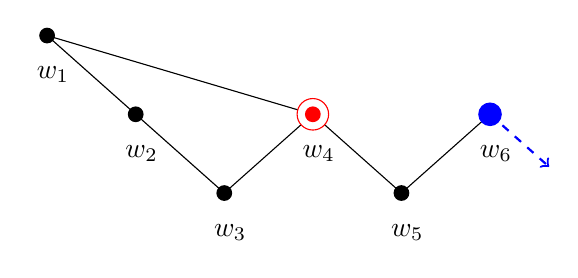
\begin{tikzpicture}
\draw (0*.75,0)-- (3*.75,-2)--(4.5*.75,-1)--(0*.75,0);
\draw(4.5*.75,-1)--(6*.75,-2)--(7.5*.75,-1);
\fill (0*.75,0) circle(.1) ;
\draw (.1*.75,-.5) node{$\displaystyle w_1$} ;%
\fill (1.5*.75,-1) circle(.1) ;
\draw (1.6*.75,-1.5) node{$\displaystyle w_2$} ;
\fill (3*.75,-2) circle(.1) ;
\draw (3.1*.75,-2.5) node{$\displaystyle w_3$} ;
\draw (4.6*.75,-1.5) node{$\displaystyle w_4$} ;
\fill[blue] (7.5*.75,-1) circle(.15) ;
\draw (6.1*.75,-2.5) node{$\displaystyle w_5$} ;
\draw (7.6*.75,-1.5) node{$\displaystyle w_6$} ;
\draw[->, blue, dashed, thick] (7.5*.75,-1)--(8.5*.75,-5/3);
\fill(6*.75,-2) circle(.1) ;
\fill[white] (4.5*.75,-1) circle(.2) ;
\fill[red] (4.5*.75,-1) circle(.1) ;
\draw[red] (4.5*.75,-1) circle(.2);
\end{tikzpicture}
 \raisebox{15mm}{$\qquad$ \scalebox{2}{$\Rightarrow$} $\qquad$}
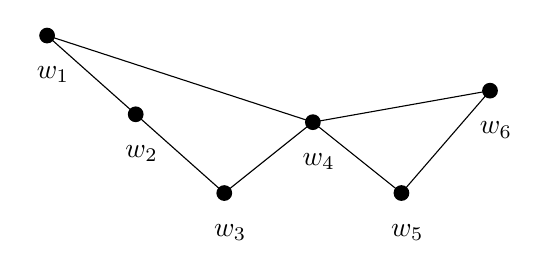
\begin{tikzpicture}
\draw (0*.75,0)-- (3*.75,-2)--(4.5*.75,-1.1)--(0*.75,0);
\draw(4.5*.75,-1.1)--(6*.75,-2)--(7.5*.75,-.7);
\fill (0*.75,0) circle(.1) ;
\draw (.1*.75,-.5) node{$\displaystyle w_1$} ;%
\fill (1.5*.75,-1) circle(.1) ;
\draw (1.6*.75,-1.5) node{$\displaystyle w_2$} ;
\fill (3*.75,-2) circle(.1) ;
\draw (3.1*.75,-2.5) node{$\displaystyle w_3$} ;
\draw (4.6*.75,-1.6) node{$\displaystyle w_4$} ;
\fill (4.5*.75,-1.1) circle(.1) ;
\fill (7.5*.75,-.7) circle(.1) ;
\draw (6.1*.75,-2.5) node{$\displaystyle w_5$} ;
\draw (7.6*.75,-1.2) node{$\displaystyle w_6$} ;
\draw (7.5*.75,-.7)--(4.5*.75,-1.1);
\fill(6*.75,-2) circle(.1) ;
\end{tikzpicture}}
\end{figure}

 The trace of $S_3$ gives us the weight polynomial:
 \begin{dmath}1+w_3+w_5+w_2w_3+w_3w_5+w_2w_3w_5+w_3w_4w_5+w_2w_3w_4w_5+w_3w_4w_5w_6+w_1w_2w_3w_4w_5+w_2w_3w_4w_5w_6+w_1w_2w_3w_4w_5w_6.\end{dmath}
 
  Plugging in the weights we obtain the following expansion formula:
 \begin{dmath*}
 x_{\gamma}=\displaystyle {\frac{x(M_-)}{\operatorname{cross}(\gamma,T)}} \rank(P_\gamma;xy)=\frac{x_1x_2x_4^2x_6}{x_1x_2x_3x_4x_5x_6}\rank(P_\gamma;xy)=\frac{x_4}{x_3x_5}+\frac{x_1x_8}{x_2x_3x_5}y_3+\frac{x_7}{x_3x_5}y_5+\frac{x_9}{x_2x_5}y_2y_3+\frac{x_1x_7x_8}{x_2x_3x_4x_5}y_3y_5+\frac{x_7x_9}{x_2x_4x_5}y_2y_3y_5+\frac{x_7x_8}{x_2x_4x_6}y_3y_4y_5+\frac{x_3x_7x_9}{x_1x_2x_4x_6}y_2y_3y_4y_5+\frac{x_8}{x_2x_6}y_3y_4y_5y_6+\frac{x_7}{x_1x_6}y_1y_2y_3y_4y_5+\frac{x_3x_9}{x_1x_2x_6}y_2y_3y_4y_5y_6+\frac{x_4}{x_1x_6}y_1y_2y_3y_4y_5y_6.
 \end{dmath*}

\end{example}
 
 \begin{example} \label{ex:double2} Here, we consider another doubly notched arc, this time with two disjoint loops in the corresponding loop graph, illustrated in Figure~\ref{doubly2}. 
 
\begin{figure}[H]
\includegraphics[width=15cm]{images/double2glued.png}
\caption{An example calculation for a doubly notched arc, from \cite{wilson}, with its corresponding labeled poset.} \label{doubly2}
\end{figure}

The source loop is that we calculated in Step 2 of the one loop case, with the corresponding matrix: 

$$S_2=\lloop_\nearrow \left( \mdo(w_1)\mdo(w_2)\mup(w_3)\mup(w_4) \right).$$

Let us know similarly calculate the target loop.

\noindent{\textbf{Step $3'$: }} Connect vertices $6$, $7$, $8$ and $9$ by up and down steps. We use the downwards arrow for vertex $9$ because we will connect it to node $6$ by adding the relation $6\preceq 9$ later.

\begin{figure}[H]
    \centering \scalebox{.8}{
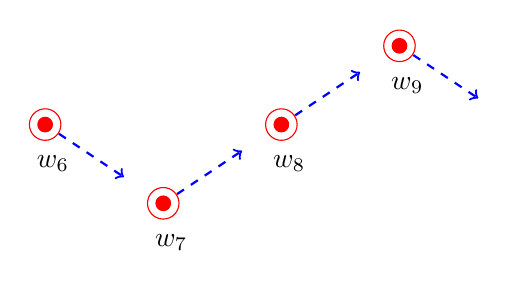
\begin{tikzpicture}
\draw[->, blue, dashed, thick] (6,0)--(7,-2/3);
\draw[->, blue, dashed, thick] (1.5,-1)--(2.5,-5/3);
\draw[->, blue, dashed, thick] (3,-2)--(4,-4/3);
\draw[->, blue, dashed, thick] (4.5,-1)--(5.5,-1/3);
\fill (6,0) circle(.2) node[white] {$9$} ;
\draw (6.1,-.5) node{$\displaystyle w_9$} ;%
\fill (1.5,-1) circle(.2) node[white] {$6$} ;
\draw (1.6,-1.5) node{$\displaystyle w_6$} ;
\fill (3,-2) circle(.2) node[white] {$7$} ;
\draw (3.1,-2.5) node{$\displaystyle w_7$} ;
\fill (4.5,-1) circle(.2) node[white] {$8$} ;
\draw (4.6,-1.5) node{$\displaystyle w_8$} ;
\fill[white] (6,0) circle(.2) ;
\fill[red] (6,0) circle(.1) ;
\draw[red] (6,0) circle(.2);
\fill[white] (1.5,-1) circle(.2) ;
\fill[red] (1.5,-1) circle(.1) ;
\draw[red] (1.5,-1) circle(.2);
\fill[white] (3,-2) circle(.2) ;
\fill[red] (3,-2) circle(.1) ;
\draw[red] (3,-2) circle(.2);
\fill[white] (4.5,-1) circle(.2) ;
\fill[red] (4.5,-1) circle(.1) ;
\draw[red] (4.5,-1) circle(.2);
\end{tikzpicture} \raisebox{15mm}{$\qquad$ \scalebox{2}{$\Rightarrow$} $\qquad$}
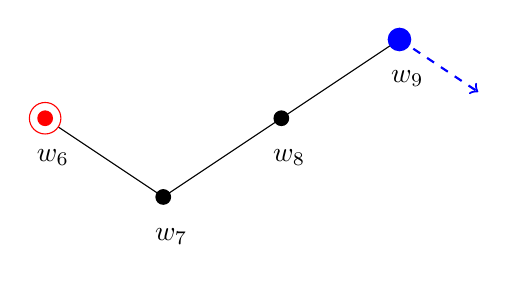
\begin{tikzpicture}
\draw (1.5,-1)-- (3,-2)--(6,0);
\draw[->, blue, dashed,thick] (6,0)--(7,-2/3);
\fill (4.5,-1) circle(.1) ;
\draw (6.1,-.5) node{$\displaystyle w_9$} ;%
\fill (1.5,-1) circle(.1) ;
\draw (1.6,-1.5) node{$\displaystyle w_6$} ;
\fill (3,-2) circle(.1) ;
\draw (3.1,-2.5) node{$\displaystyle w_7$} ;
\fill[blue] (6,0) circle(.15);
\draw (4.6,-1.5) node{$\displaystyle w_8$} ;
\fill[white] (1.5,-1) circle(.2) ;
\fill[red] (1.5,-1) circle(.1) ;
\draw[red] (1.5,-1) circle(.2);
\end{tikzpicture}}
\end{figure}

The correponding matrix is:

$$S_{3'}= \mdo(w_6)\mup(w_7)\mup(w_8)\mdo(w_9)= \mdom{w_6}\mupm{w_7}\mupm{w_8}\mdom{w_9}.$$

\noindent{\textbf{Step $4'`$: }} Connect vertices $6$ and $9$ using the $\rloop$ operation so that the connections remain on the target (left) side:
\begin{figure}[H]
    \centering \scalebox{.8}{
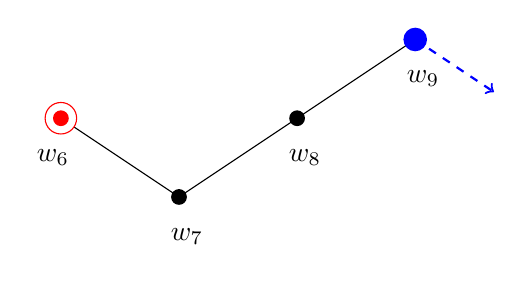
\begin{tikzpicture}
\draw (1.5,-1)-- (3,-2)--(6,0);
\draw[->, blue, dashed,thick] (6,0)--(7,-2/3);
\fill (4.5,-1) circle(.1) ;
\draw (6.1,-.5) node{$\displaystyle w_9$} ;%
\fill (1.5,-1) circle(.1) ;
\draw (1.4,-1.5) node{$\displaystyle w_6$} ;
\fill (3,-2) circle(.1) ;
\draw (3.1,-2.5) node{$\displaystyle w_7$} ;
\fill[blue] (6,0) circle(.15);
\draw (4.6,-1.5) node{$\displaystyle w_8$} ;
\fill[white] (1.5,-1) circle(.2) ;
\fill[red] (1.5,-1) circle(.1) ;
\draw[red] (1.5,-1) circle(.2);
\end{tikzpicture} \raisebox{15mm}{$\qquad$ \scalebox{2}{$\Rightarrow$} $\qquad$}
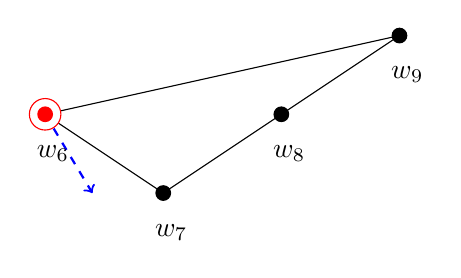
\begin{tikzpicture}
\draw (1.5,-1)-- (3,-2)--(6,0)--(1.5,-1);
\draw[->, blue, dashed,thick] (1.5,-1)--(2.1,-2);
\fill (4.5,-1) circle(.1) ;
\draw (6.1,-.5) node{$\displaystyle w_9$} ;%
\fill (1.5,-1) circle(.1) ;
\draw (1.6,-1.5) node{$\displaystyle w_6$} ;
\fill (3,-2) circle(.1) ;
\draw (3.1,-2.5) node{$\displaystyle w_7$} ;
\fill (6,0) circle(.1);
\draw (4.6,-1.5) node{$\displaystyle w_8$} ;
\fill[white] (1.5,-1) circle(.2) ;
\fill[red] (1.5,-1) circle(.1) ;
\draw[red] (1.5,-1) circle(.2);
\end{tikzpicture}}
\end{figure}

We get the following matrix:
$$S_{4'}=\rloop\left( \mdo(w_6)\mup(w_7)\mup(w_8)\mdo(w_9) \right)=\rloop\left( \mdom{w_6}\mupm{w_7}\mupm{w_8}\mdom{w_9} \right).$$

\noindent{\textbf{Step $5'$: }} Finally, connect the pieces together adding an up step for vertex $5$ in the middle to get the full poset.



\begin{figure}[H]
    \centering \scalebox{.8}{
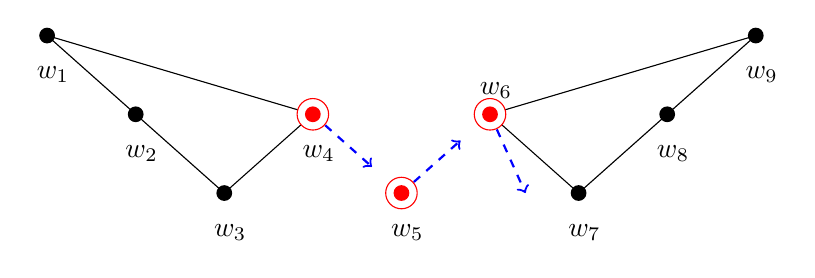
\begin{tikzpicture}
\draw (0*.75,0)-- (3*.75,-2)--(4.5*.75,-1)--(0*.75,0);
%\draw[->, blue, dotted] (4.5*.75,-1)--(5.5*.75,-1/3);
\draw[->, blue, dashed, thick] (4.5*.75,-1)--(5.5*.75,-5/3);
%\draw[black,->,thick] (5.2*.75,-3/4)--(5.2*.75,-5/4);
\fill (0*.75,0) circle(.1) ;
\draw (.1*.75,-.5) node{$\displaystyle w_1$} ;%
\fill (1.5*.75,-1) circle(.1) ;
\draw (1.6*.75,-1.5) node{$\displaystyle w_2$} ;
\fill (3*.75,-2) circle(.1) ;
\draw (3.1*.75,-2.5) node{$\displaystyle w_3$} ;
\draw (4.6*.75,-1.5) node{$\displaystyle w_4$} ;
\fill[white] (4.5*.75,-1) circle(.2) ;
\fill[red] (4.5*.75,-1) circle(.1) ;
\draw[red] (4.5*.75,-1) circle(.2);
\draw (6.1*.75,-2.5) node{$\displaystyle w_5$} ;
\draw[->, blue, dashed, thick] (6*.75,-2)--(7*.75,-4/3);
\fill[white] (6*.75,-2) circle(.2) ;
\fill[red] (6*.75,-2) circle(.1) ;
\draw[red] (6*.75,-2) circle(.2);
\draw (7.5*.75,-1)-- (9*.75,-2)--(12*.75,0)--(7.5*.75,-1);
\draw[->, blue, dashed,thick] (7.5*.75,-1)--(8.1*.75,-2);
\fill (10.5*.75,-1) circle(.1) ;
\draw (12.1*.75,-.5) node{$\displaystyle w_9$} ;%
\fill (7.5*.75,-1) circle(.1) ;
\draw (7.6*.75,-.7) node{$\displaystyle w_6$} ;
\fill (9*.75,-2) circle(.1) ;
\draw (9.1*.75,-2.5) node{$\displaystyle w_7$} ;
\fill (12*.75,0) circle(.1);
\draw (10.6*.75,-1.5) node{$\displaystyle w_8$} ;
\fill[white] (7.5*.75,-1) circle(.2) ;
\fill[red] (7.5*.75,-1) circle(.1) ;
\draw[red] (7.5*.75,-1) circle(.2);
\end{tikzpicture}
 \raisebox{15mm}{$\,$ \scalebox{2}{$\Rightarrow$} $\,$}
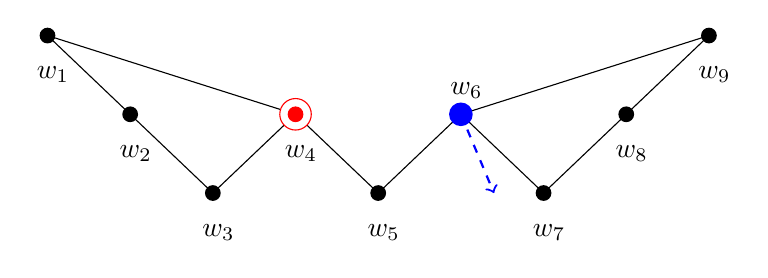
\begin{tikzpicture}
\draw (0*.7,0)-- (3*.7,-2)--(4.5*.7,-1)--(0*.7,0);
%\draw[->, blue, dotted] (4.5*.7,-1)--(5.5*.7,-1/3);
%\draw[->, blue, dashed, thick] (4.5*.7,-1)--(5.5*.7,-5/3);
%\draw[black,->,thick] (5.2*.7,-3/4)--(5.2*.7,-5/4);
\fill (0*.7,0) circle(.1) ;
\draw (.1*.7,-.5) node{$\displaystyle w_1$} ;%
\fill (1.5*.7,-1) circle(.1) ;
\draw (1.6*.7,-1.5) node{$\displaystyle w_2$} ;
\fill (3*.7,-2) circle(.1) ;
\draw (3.1*.7,-2.5) node{$\displaystyle w_3$} ;
\draw (4.6*.7,-1.5) node{$\displaystyle w_4$} ;
\draw (6.1*.7,-2.5) node{$\displaystyle w_5$} ;
%\draw[->, blue, dashed, thick] (6*.7,-2)--(7*.7,-4/3);
\draw  (4.5*.7,-1)--(6*.7,-2) --(7.5*.7,-1);
\fill (6*.7,-2) circle(.1) ;
\draw (7.5*.7,-1)-- (9*.7,-2)--(12*.7,0)--(7.5*.7,-1);
\draw[->, blue, dashed,thick] (7.5*.7,-1)--(8.1*.7,-2);
\fill (10.5*.7,-1) circle(.1) ;
\draw (12.1*.7,-.5) node{$\displaystyle w_9$} ;%
\fill (7.5*.7,-1) circle(.1) ;
\draw (7.6*.7,-.7) node{$\displaystyle w_6$} ;
\fill (9*.7,-2) circle(.1) ;
\draw (9.1*.7,-2.5) node{$\displaystyle w_7$} ;
\fill (12*.7,0) circle(.1);
\draw (10.6*.7,-1.5) node{$\displaystyle w_8$} ;
\fill[blue] (7.5*.7,-1) circle(.15) ;
\fill[white] (4.5*.7,-1) circle(.2) ;
\fill[red] (4.5*.7,-1) circle(.1) ;
\draw[red] (4.5*.7,-1) circle(.2);
\end{tikzpicture}}
\end{figure}


\begin{align*}
S_{5'}=S_2\cdot \mup(w_5) \cdot S_{4'} = \lloop_\nearrow \left( \mdo(w_1)\mdo(w_2)\mup(w_3)\mup(w_4) \right)\cdot \mup(w_5) \cdot \rloop\left( \mdo(w_6)\mup(w_7)\mup(w_8)\mdo(w_9) \right).
\end{align*}

The upper left entry of the matrix gives us the following rank polynomial

\begin{dmath*}
\rank(P_\gamma;w)=
1 + w_3 + w_5 + w_7 + w_2w_3 + w_3w_5 + w_3w_7 + w_5w_7 + w_7w_8 + w_2w_3w_5 + w_3w_4w_5 + w_2w_3w_7 + w_3w_5w_7 + w_5w_6w_7 + w_3w_7w_8 + w_5w_7w_8 + w_2w_3w_4w_5 + w_2w_3w_5w_7 + w_3w_4w_5w_7 + w_3w_5w_6w_7 + w_2w_3w_7w_8 + w_3w_5w_7w_8 + w_5w_6w_7w_8 + w_1w_2w_3w_4w_5 + w_2w_3w_4w_5w_7 + w_2w_3w_5w_6w_7 + w_3w_4w_5w_6w_7 + w_2w_3w_5w_7w_8 + w_3w_4w_5w_7w_8 + w_3w_5w_6w_7w_8 + w_5w_6w_7w_8w_9  + w_1w_2w_3w_4w_5w_7 + w_2w_3w_4w_5w_6w_7 + w_2w_3w_4w_5w_7w_8 + w_2w_3w_5w_6w_7w_8 + w_3w_4w_5w_6w_7w_8 + w_3w_5w_6w_7w_8w_9  + w_1w_2w_3w_4w_5w_6w_7 + w_1w_2w_3w_4w_5w_7w_8 + w_2w_3w_4w_5w_6w_7w_8 + w_2w_3w_5w_6w_7w_8w_9 + w_3w_4w_5w_6w_7w_8w_9+ w_1w_2w_3w_4w_5w_6w_7w_8 + w_2w_3w_4w_5w_6w_7w_8w_9+w_1w_2w_3w_4w_5w_6w_7w_8w_9.
\end{dmath*}



 \end{example}
 
 \subsection{Self-folded Triangle}
  In this subsection, we include an example with a self-folded triangle in the triangulation. See \cite[Figure 8]{wilson} for the tile configuration of the self-folded triangle. After we obtain the snake graph, the computation of cluster variable via matrices is the same as above examples. 
  
\begin{figure}[H]
\includegraphics[width=9.7cm]{images/self-folded.pdf}
\caption{An example with a self folded triangle and the corresponding fence poset} \label{selfi}
\end{figure}

  

\begin{rmk} If we have an arc ending at a puncture with a self-folded triangle, we do not have to consider any tagging on that end. 
\end{rmk}

%\section{Extras, Future Directions}


%\ezgi{We can add that for one loop we do not need the concept of good matchings as a remark.
%Also discuss how to get the labeled fence poset directly from the triangulation.}



\bibliographystyle{alpha}
\bibliography{mainCE}

\end{document}
%%%%%%%%%%%%%%%%%%%%%%%%%%%%%%%%%%%%%%%%%%%%%%%%%%%%%%%55




%%%%%%%%%%%%%%%%%%%%%%%%%%%%%%%%%%%%%%%%%%%%%%%%%%%%%%%%%%%%%%%%%%%%%%%%%%%%%%


